\documentclass[a4paper, 12pt]{article}

\title{
{\large Topological Data Analysis -- group project} \\
	\vspace{3mm}
	\hrule
	\vspace{3mm}
Sensors
	\vspace{3mm}
	\hrule
}

\author{
	Nejc Ki\v sek,
	\v Zan Klane\v cek
}

\usepackage[utf8x]{inputenc}
\usepackage{float}
\usepackage{graphicx}
\usepackage{subcaption}
\usepackage{geometry}
\usepackage{amsfonts}
\usepackage{amsmath}
\usepackage{amssymb}


\begin{document}
\maketitle


\section{Introduction}
In this project we are trying to find optimal parameters for a sensor network which covers the whole surface of the earth. The network is determined by two parameters: 
\begin{itemize}
	\item \textbf{$r$}, which is the distance over which the sensors can communicate with each other -- each sensor can communicate with other, if they are at most $r$ away.
	\item \textbf{$R$}, which is the radius of the surrounding are in shape of a circle where the sensor can gather data.
\end{itemize}

Given the coordinates of each sensor, we had to determine lowest possible parameters $r$ and $R$ so that:The parameters has to be as low as possible (to reduce the cost of sensors), the whole network has to be connected and the whole surface of the Earth has to be covered.

\begin{figure}[H]
        \centering
        \makebox[\linewidth][c]{
        	\centering
            \begin{subfigure}[b]{0.55\textwidth}
                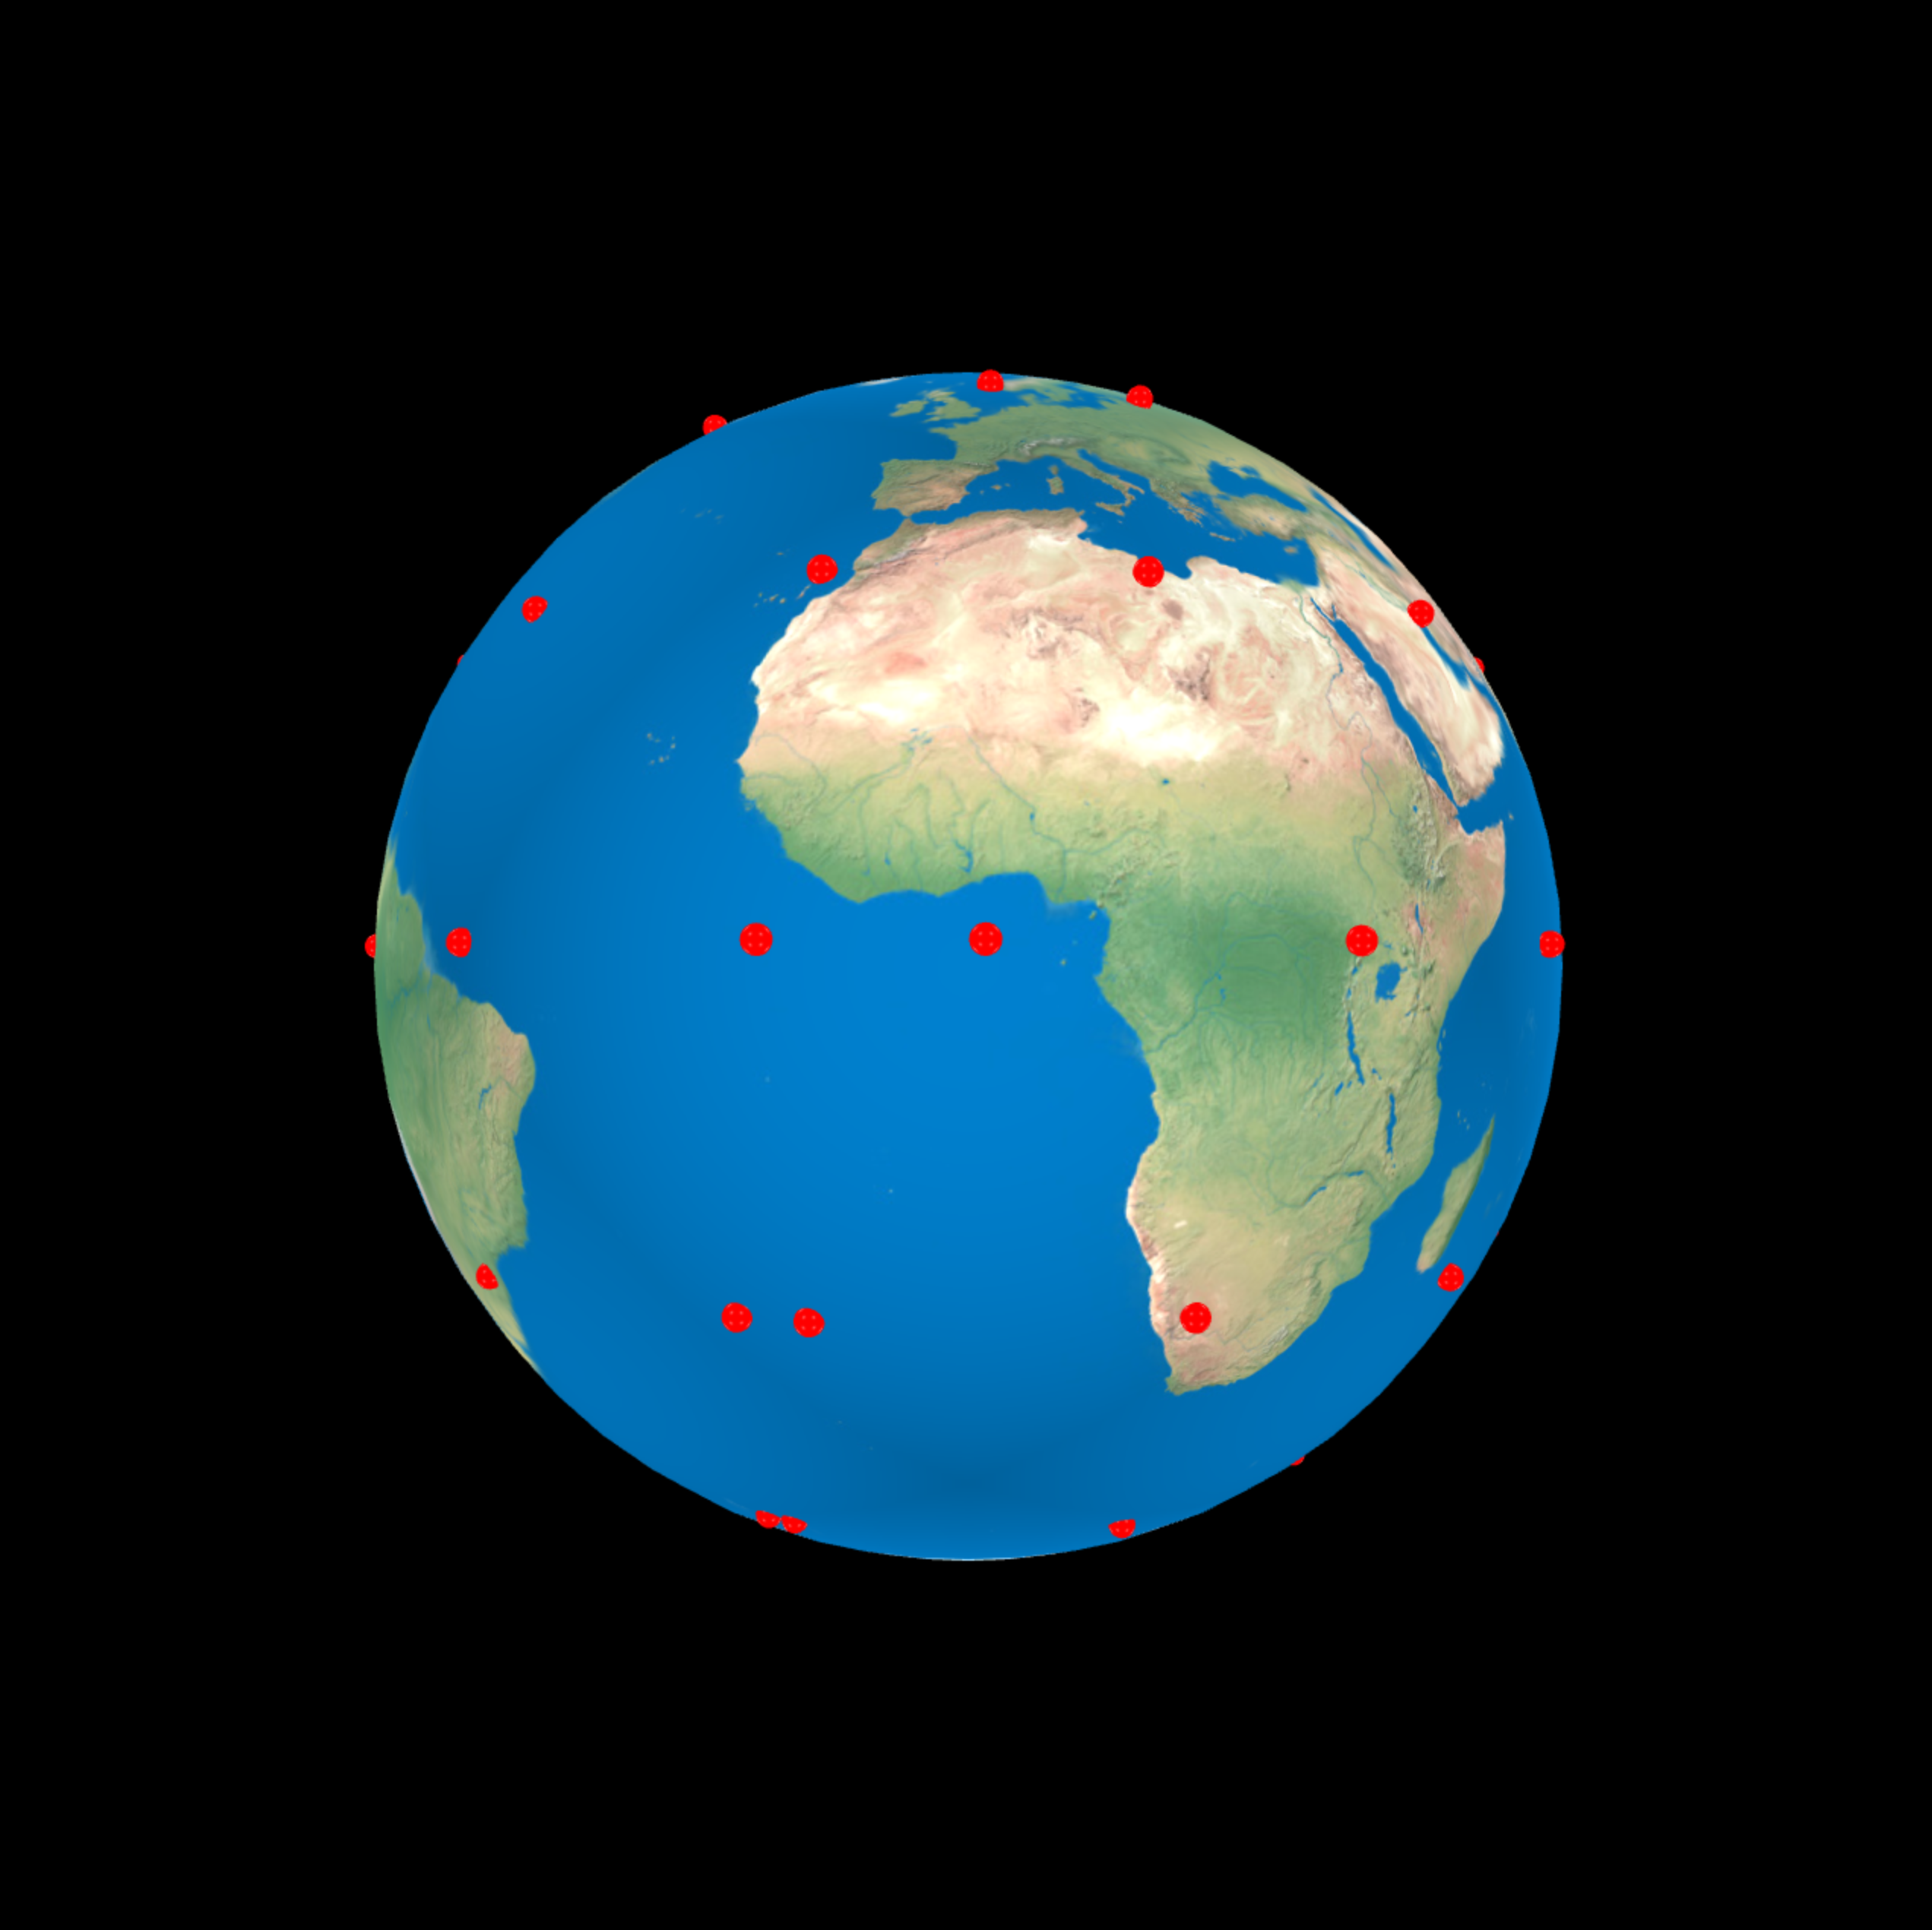
\includegraphics[width=\textwidth]{../images/sensors01}
                \caption{sensors01.txt}
            \end{subfigure}
            \begin{subfigure}[b]{0.55\textwidth}
                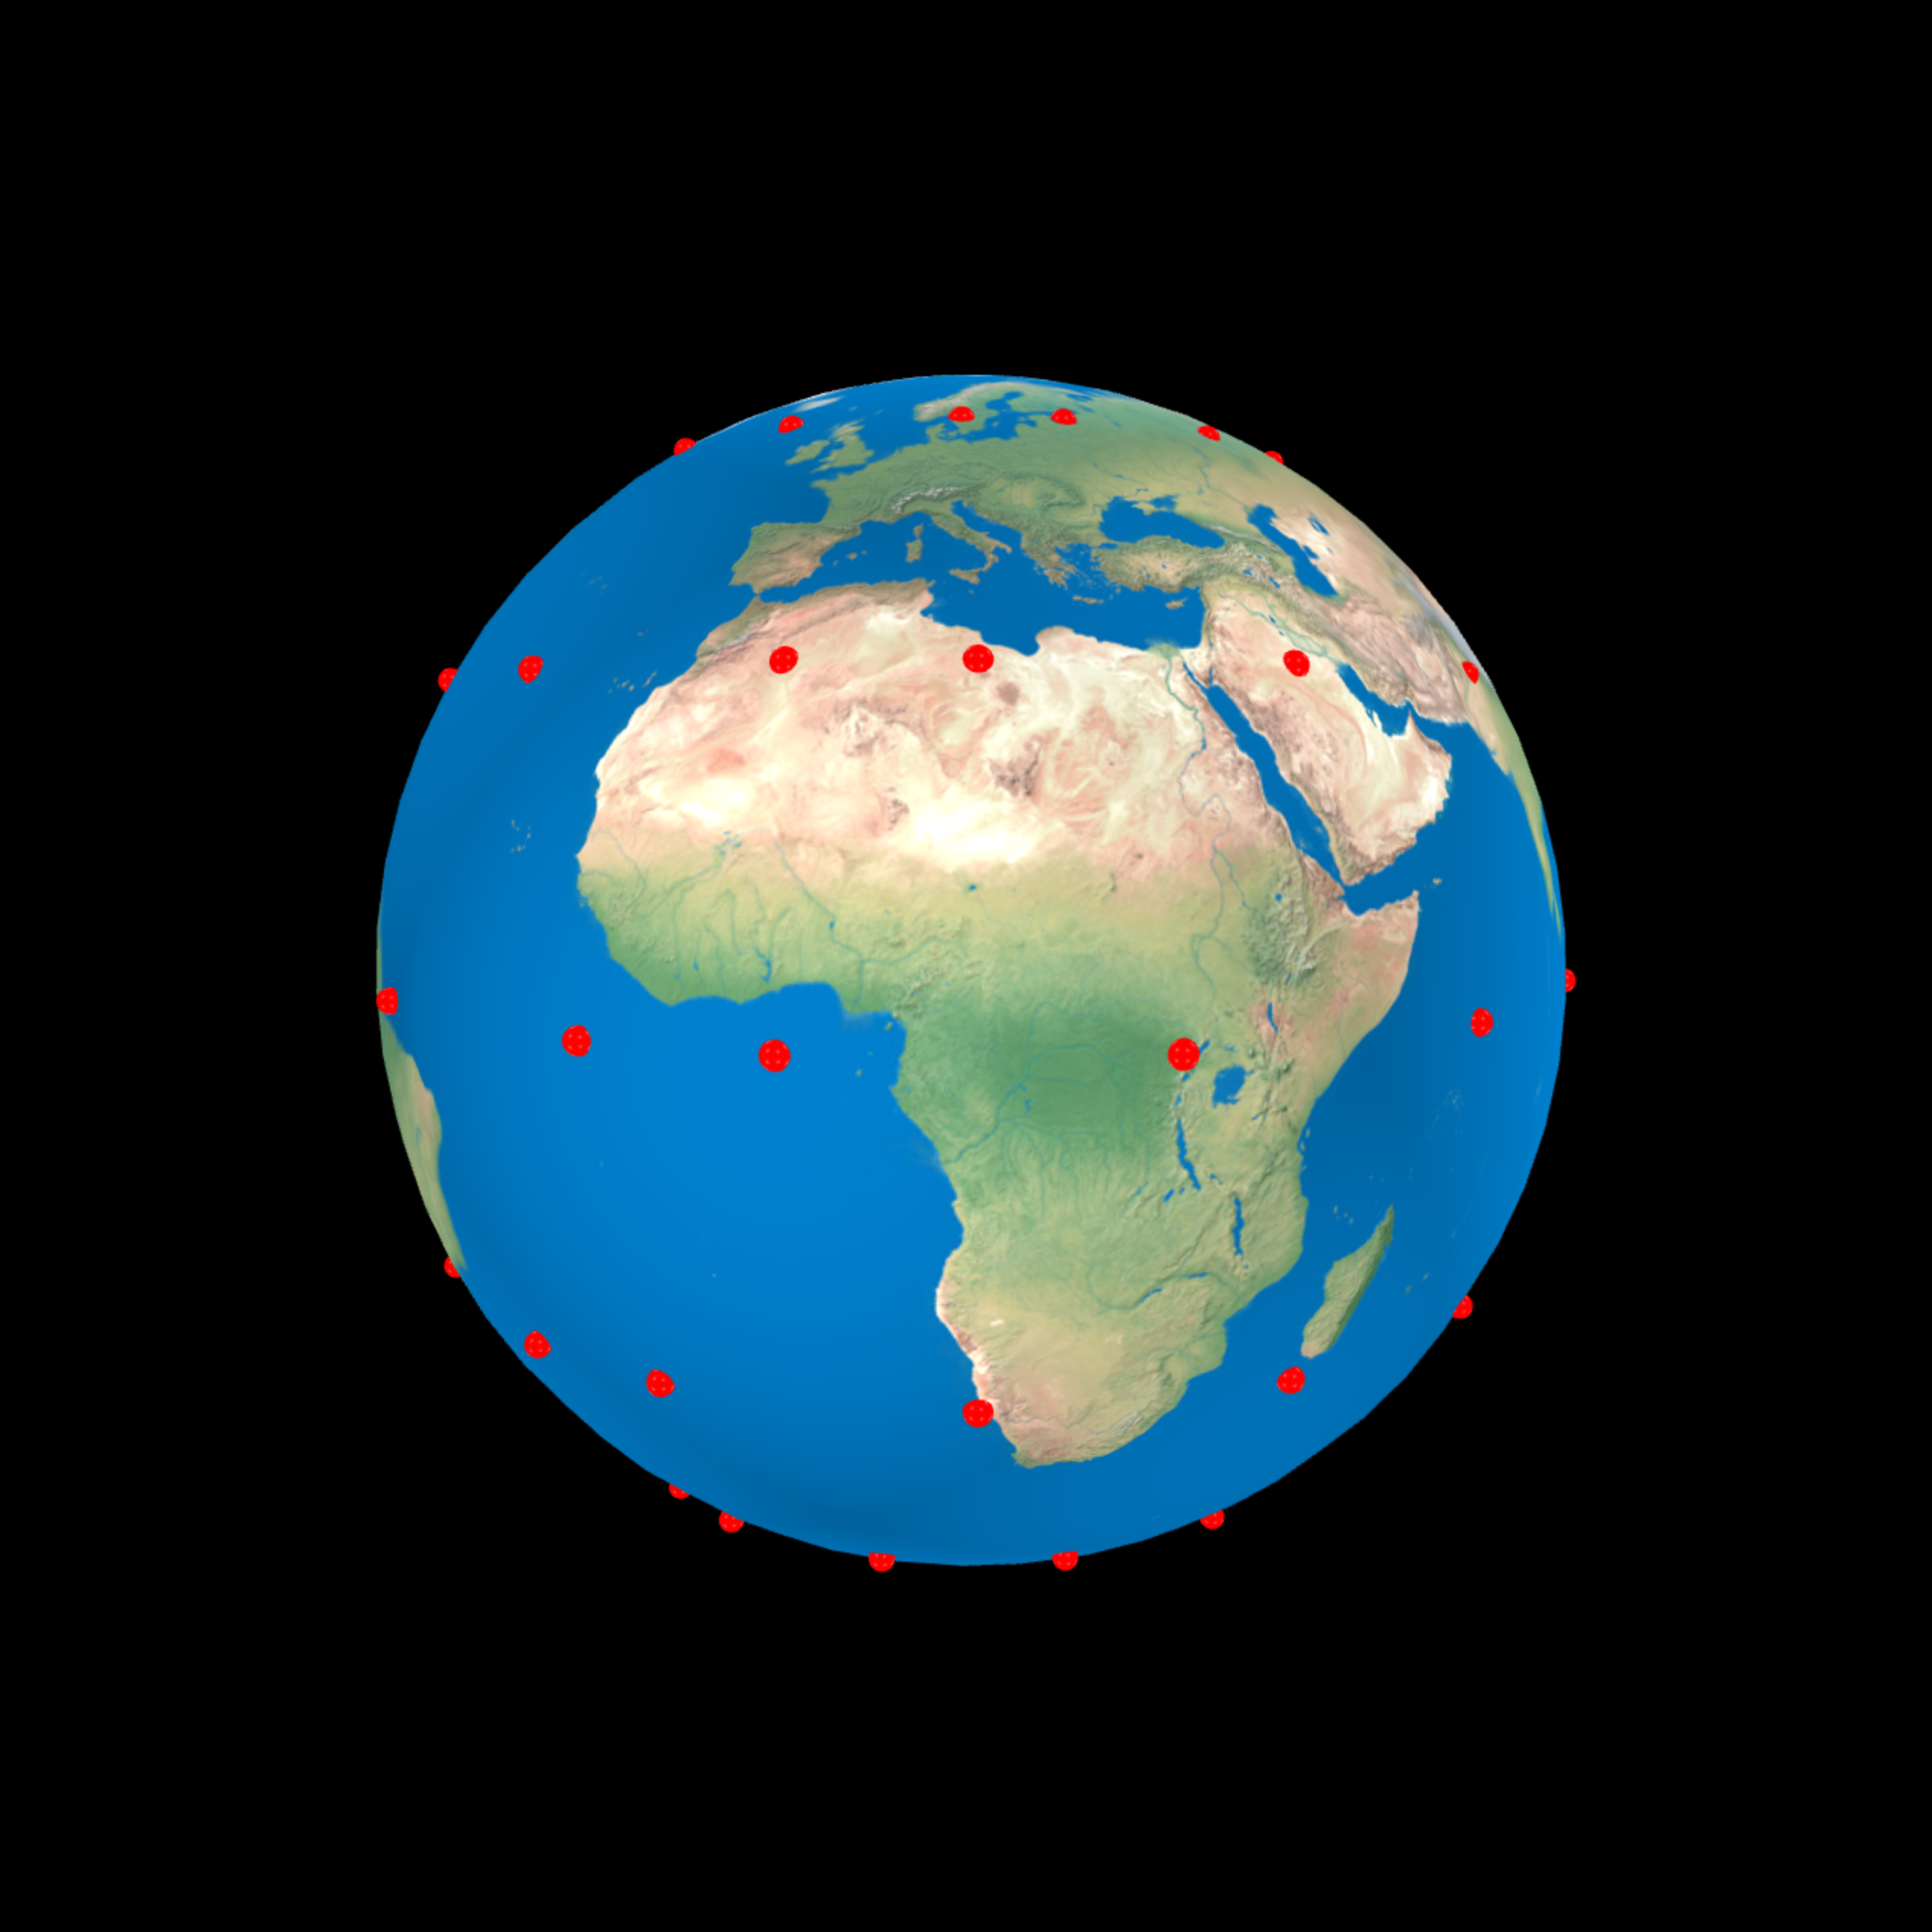
\includegraphics[width=\textwidth]{../images/sensors02}
                \caption{sensors02.txt}
            \end{subfigure}
        }
        \caption{Locations of the sensors}
\end{figure}

\section{Connectivity}
TODO: VR complex, increasing $r$ until we get 1 component. 

\begin{figure}[H]
        \centering
        \makebox[\linewidth][c]{
        	\centering
            \begin{subfigure}[b]{0.6\textwidth}
                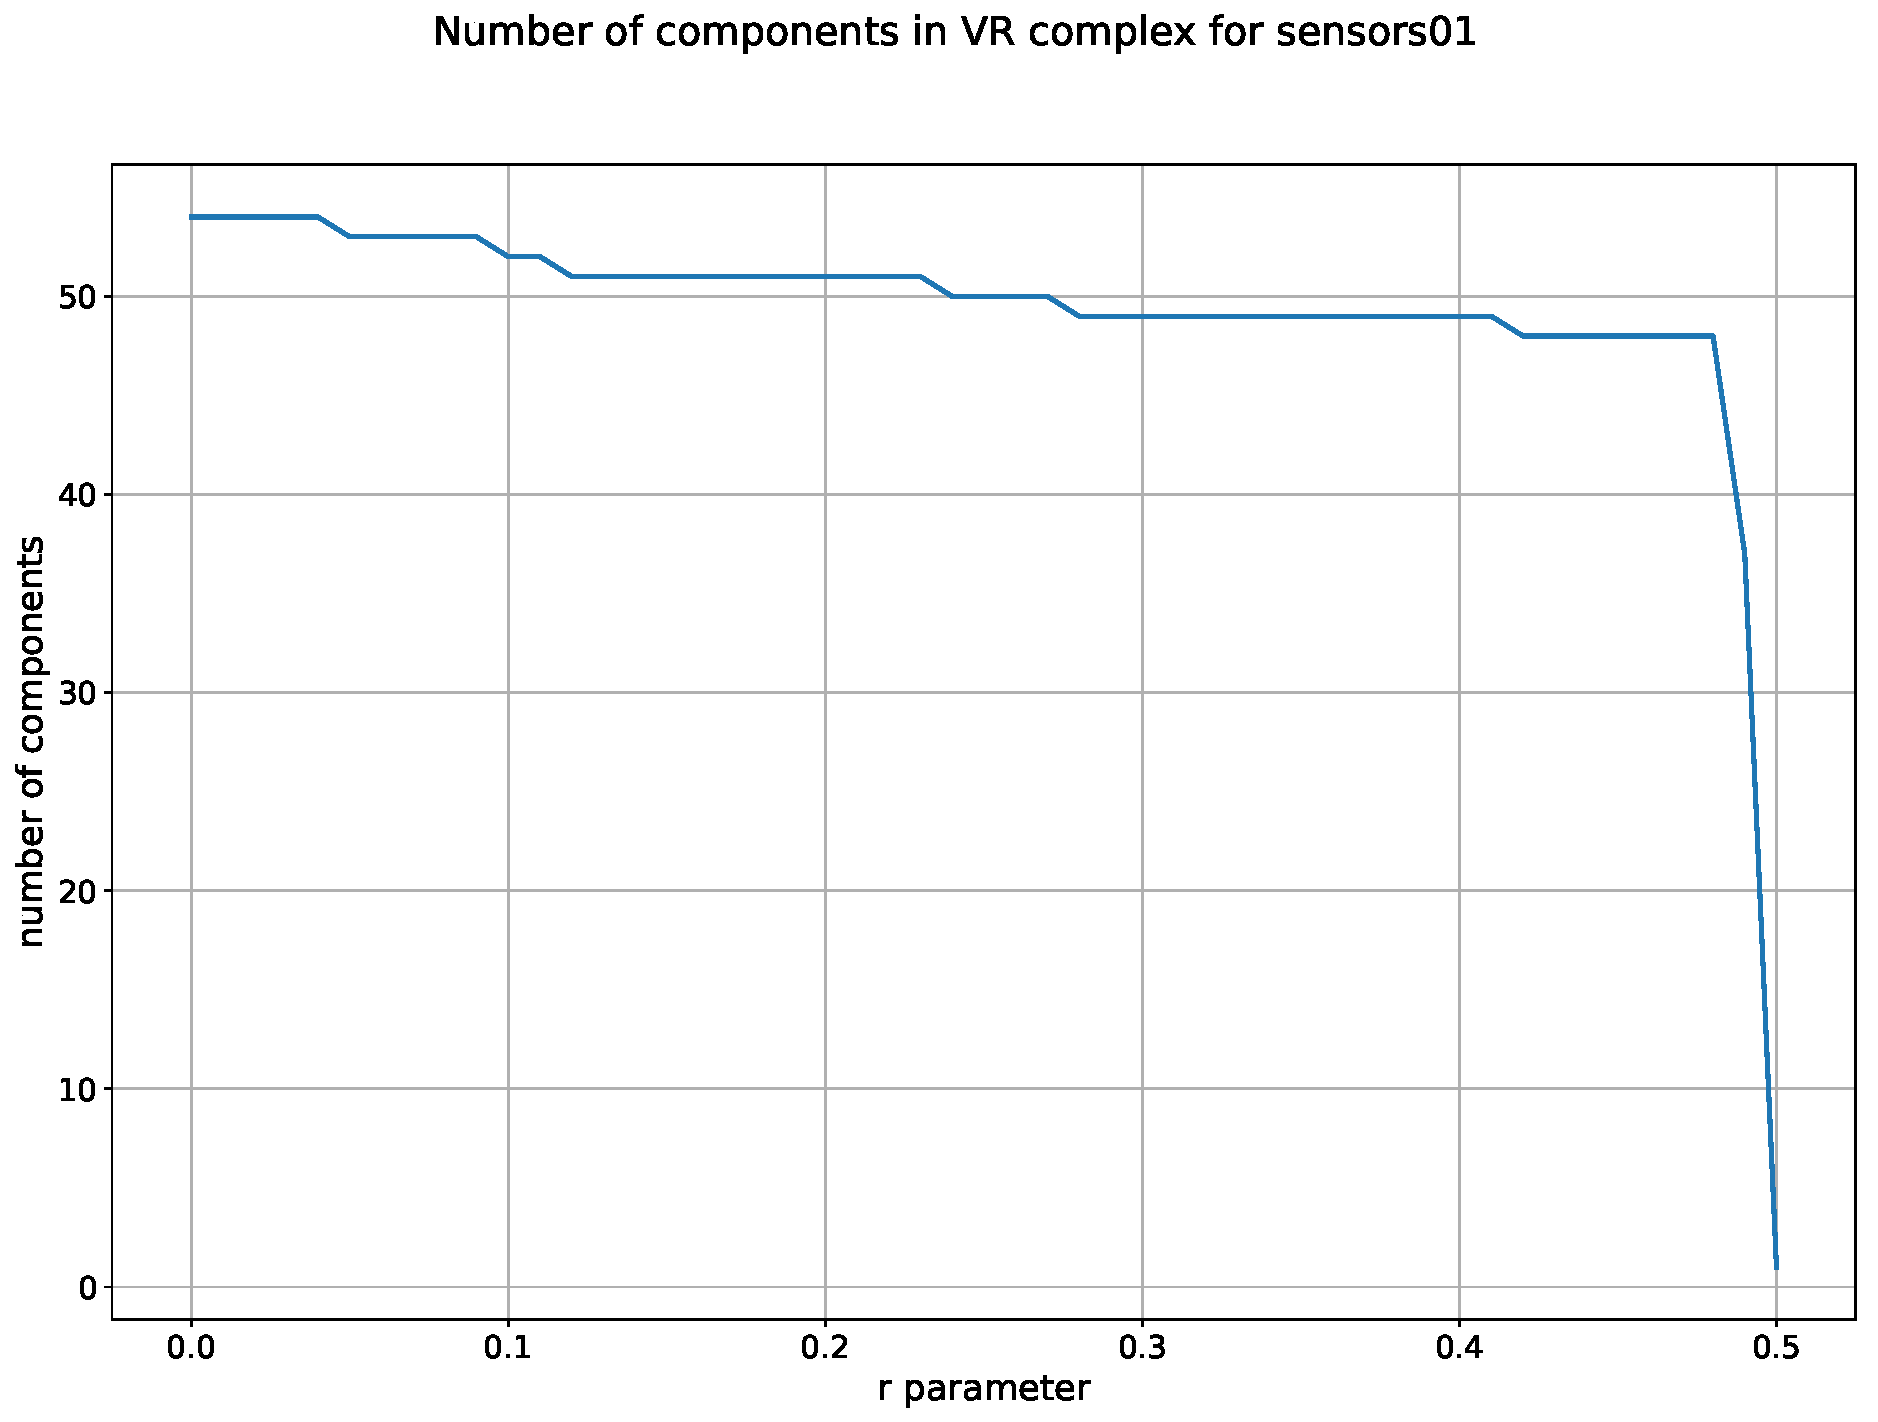
\includegraphics[width=\textwidth]{../images/plot_vr_sensors01}
            \end{subfigure}
            \begin{subfigure}[b]{0.6\textwidth}
                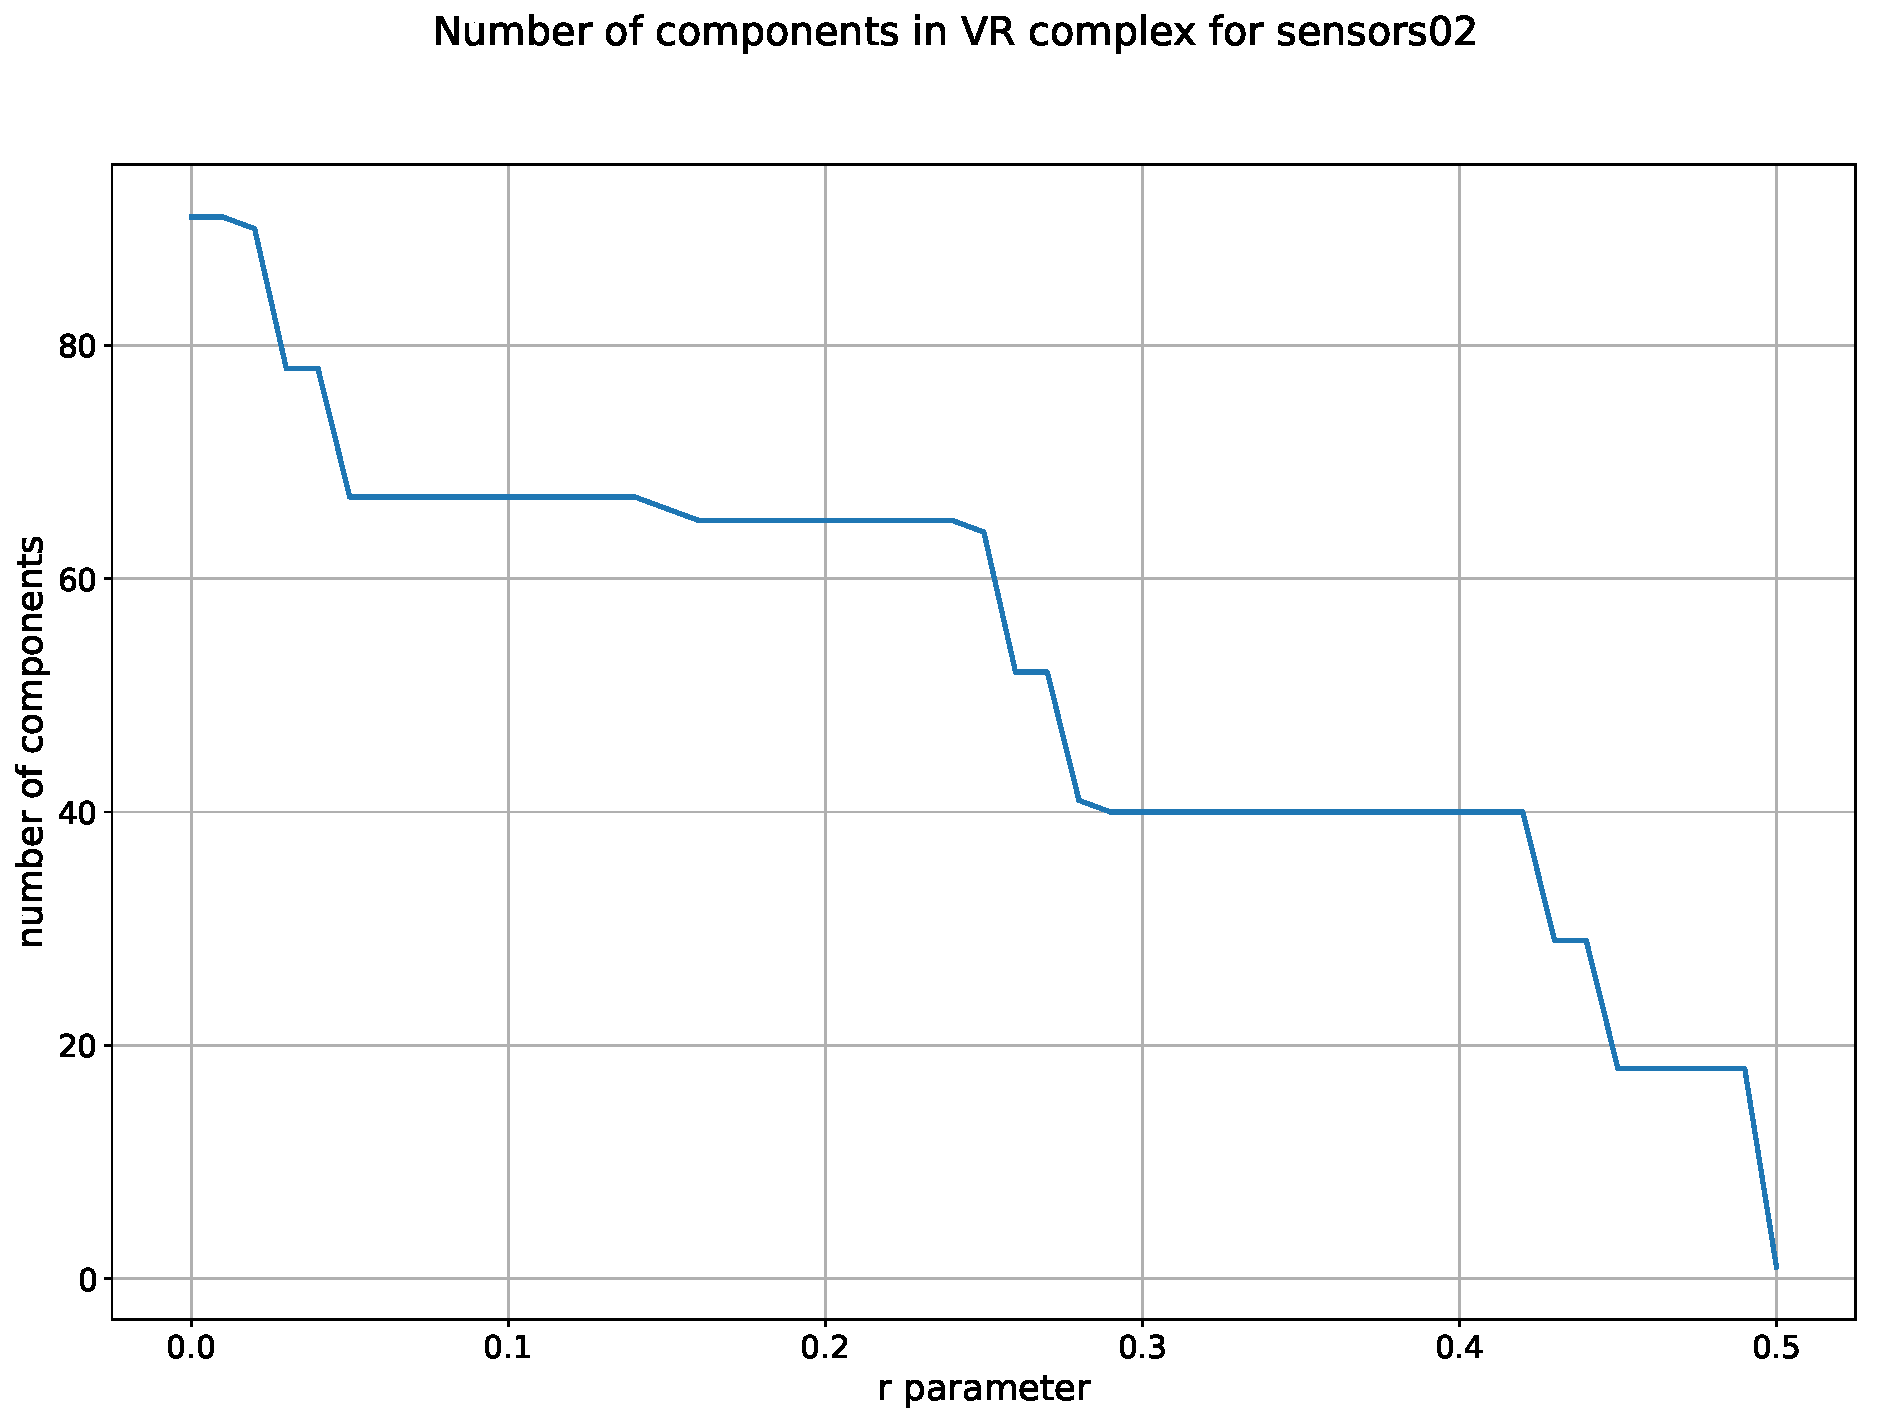
\includegraphics[width=\textwidth]{../images/plot_vr_sensors02}
            \end{subfigure}
        }
        \caption{Number of components as we increase the $r$ parameter}
\end{figure}

TODO: malo komentarja na graf

\begin{figure}[H]
        \centering
        \makebox[\linewidth][c]{
        	\centering
            \begin{subfigure}[b]{0.55\textwidth}
                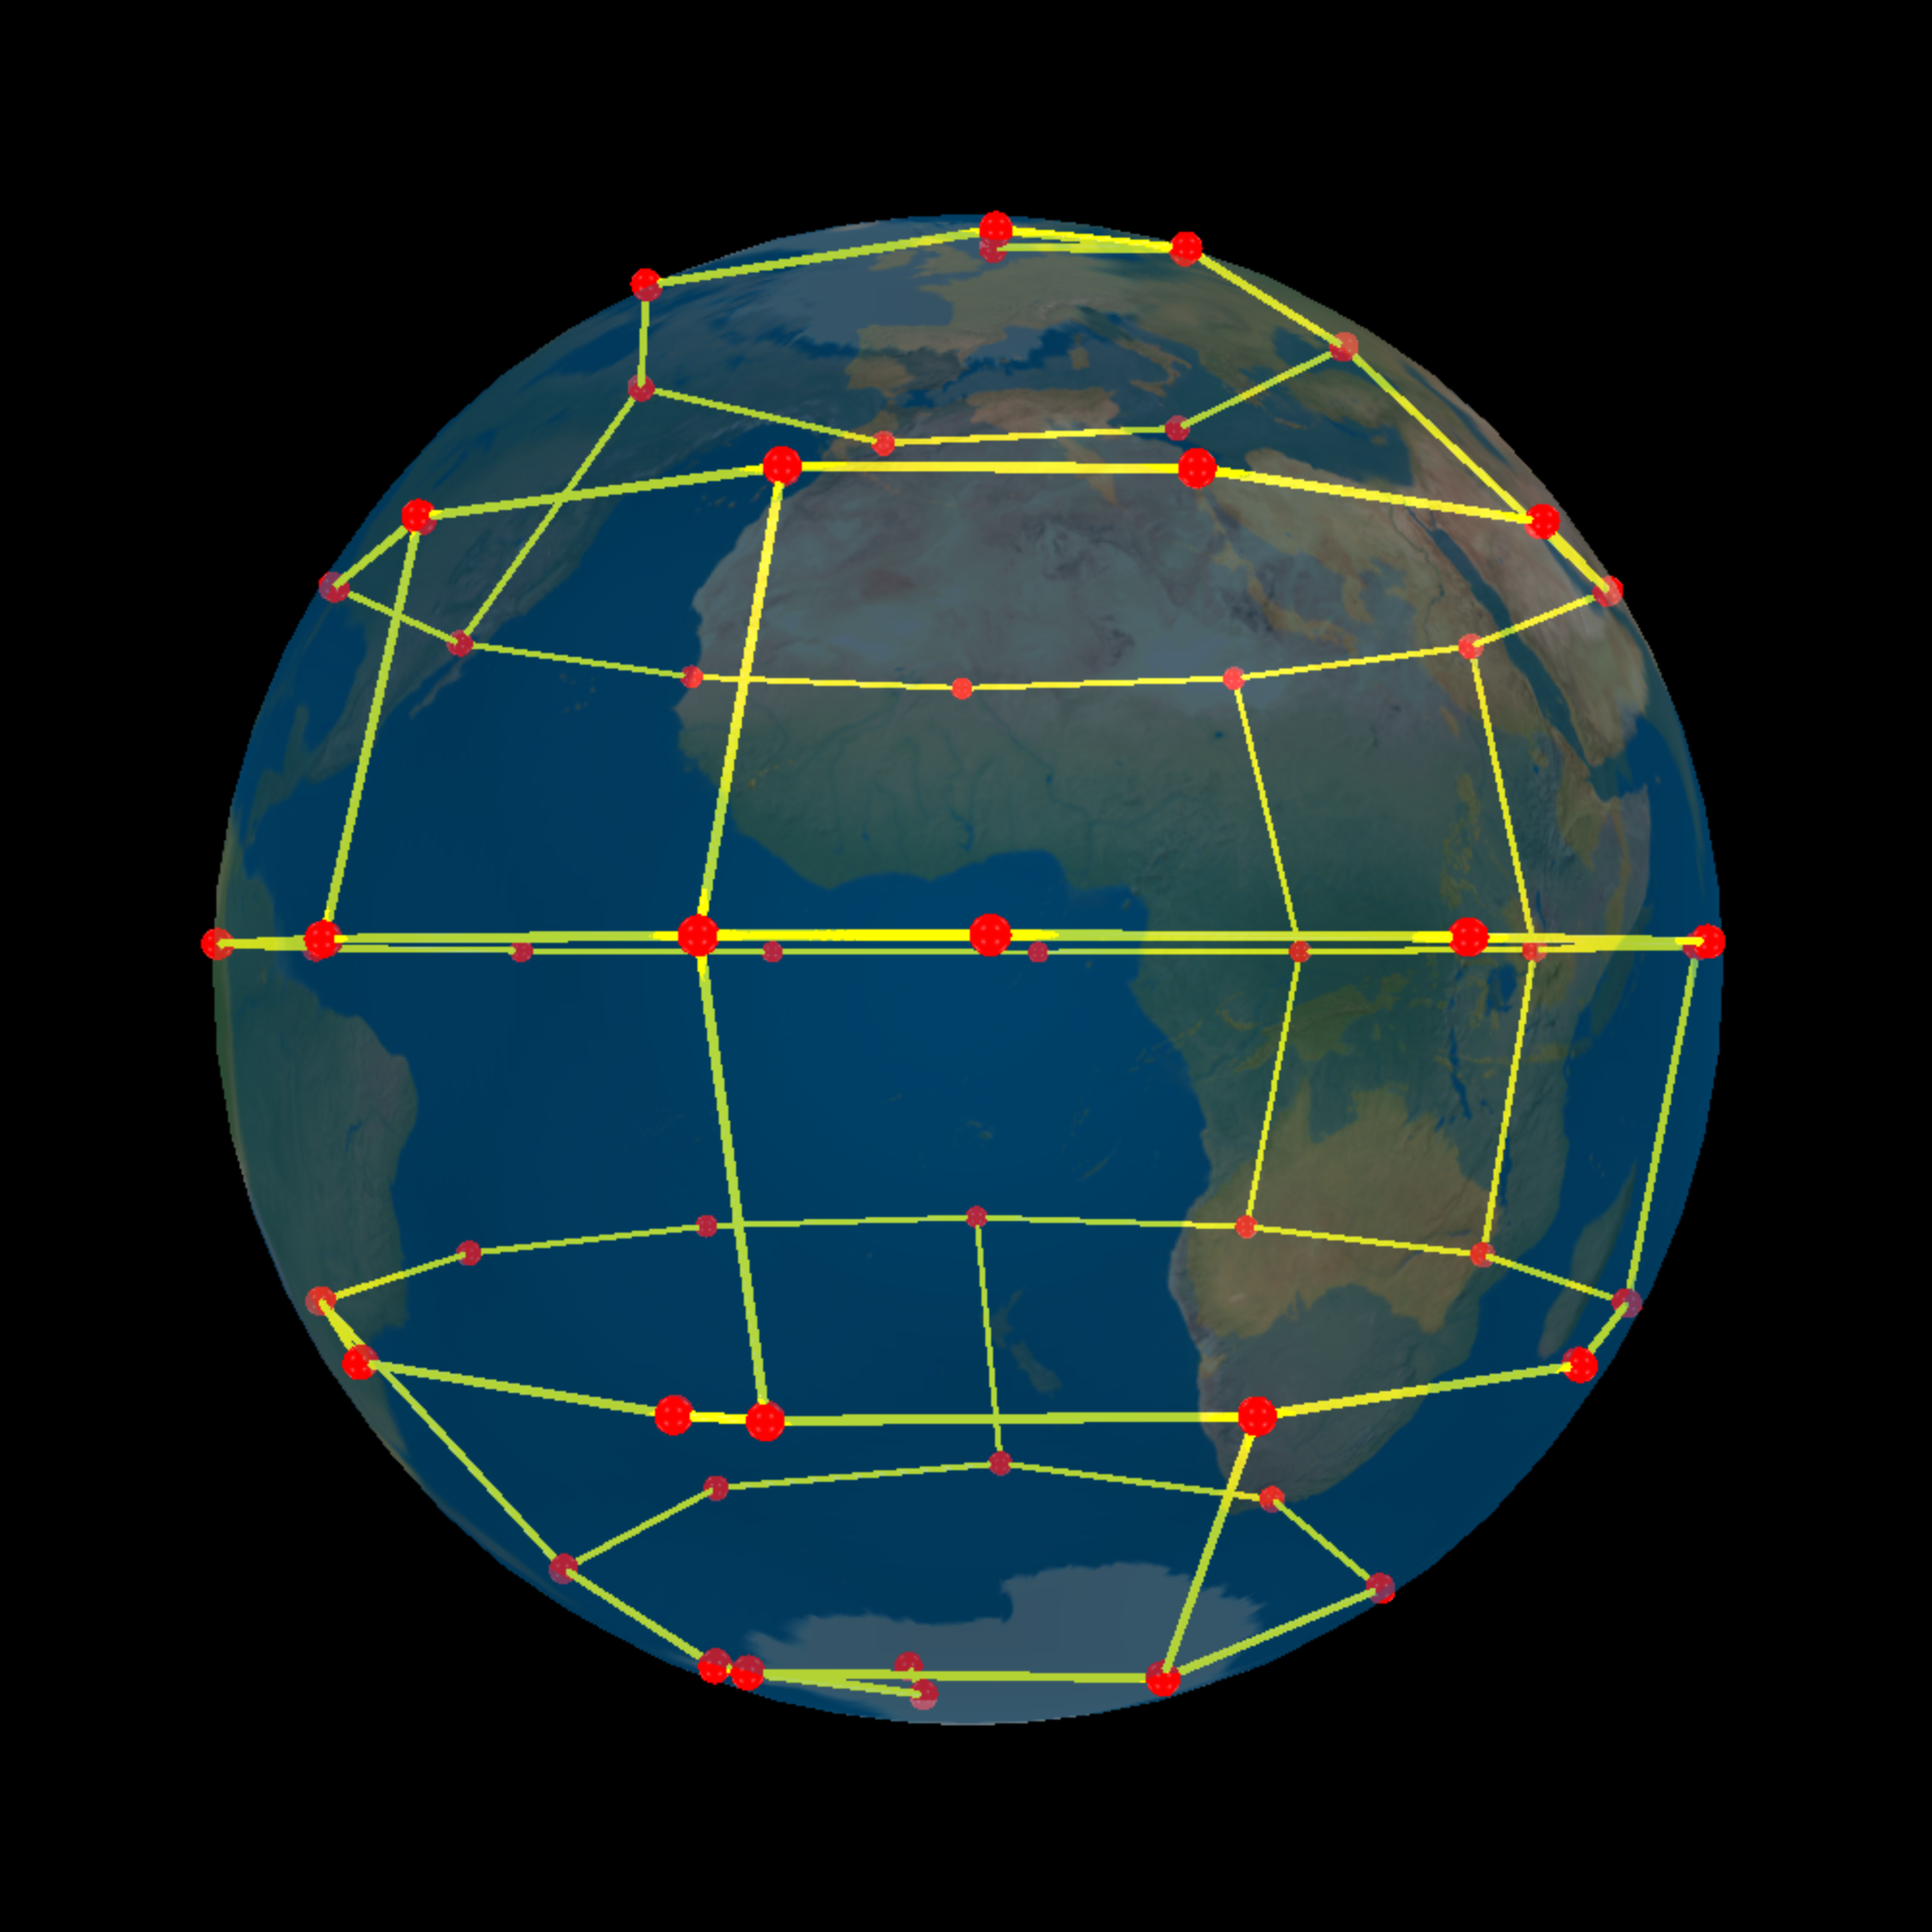
\includegraphics[width=\textwidth]{../images/connections01}
                \caption{sensors01.txt ($r=0.5$)}
            \end{subfigure}
            \begin{subfigure}[b]{0.55\textwidth}
                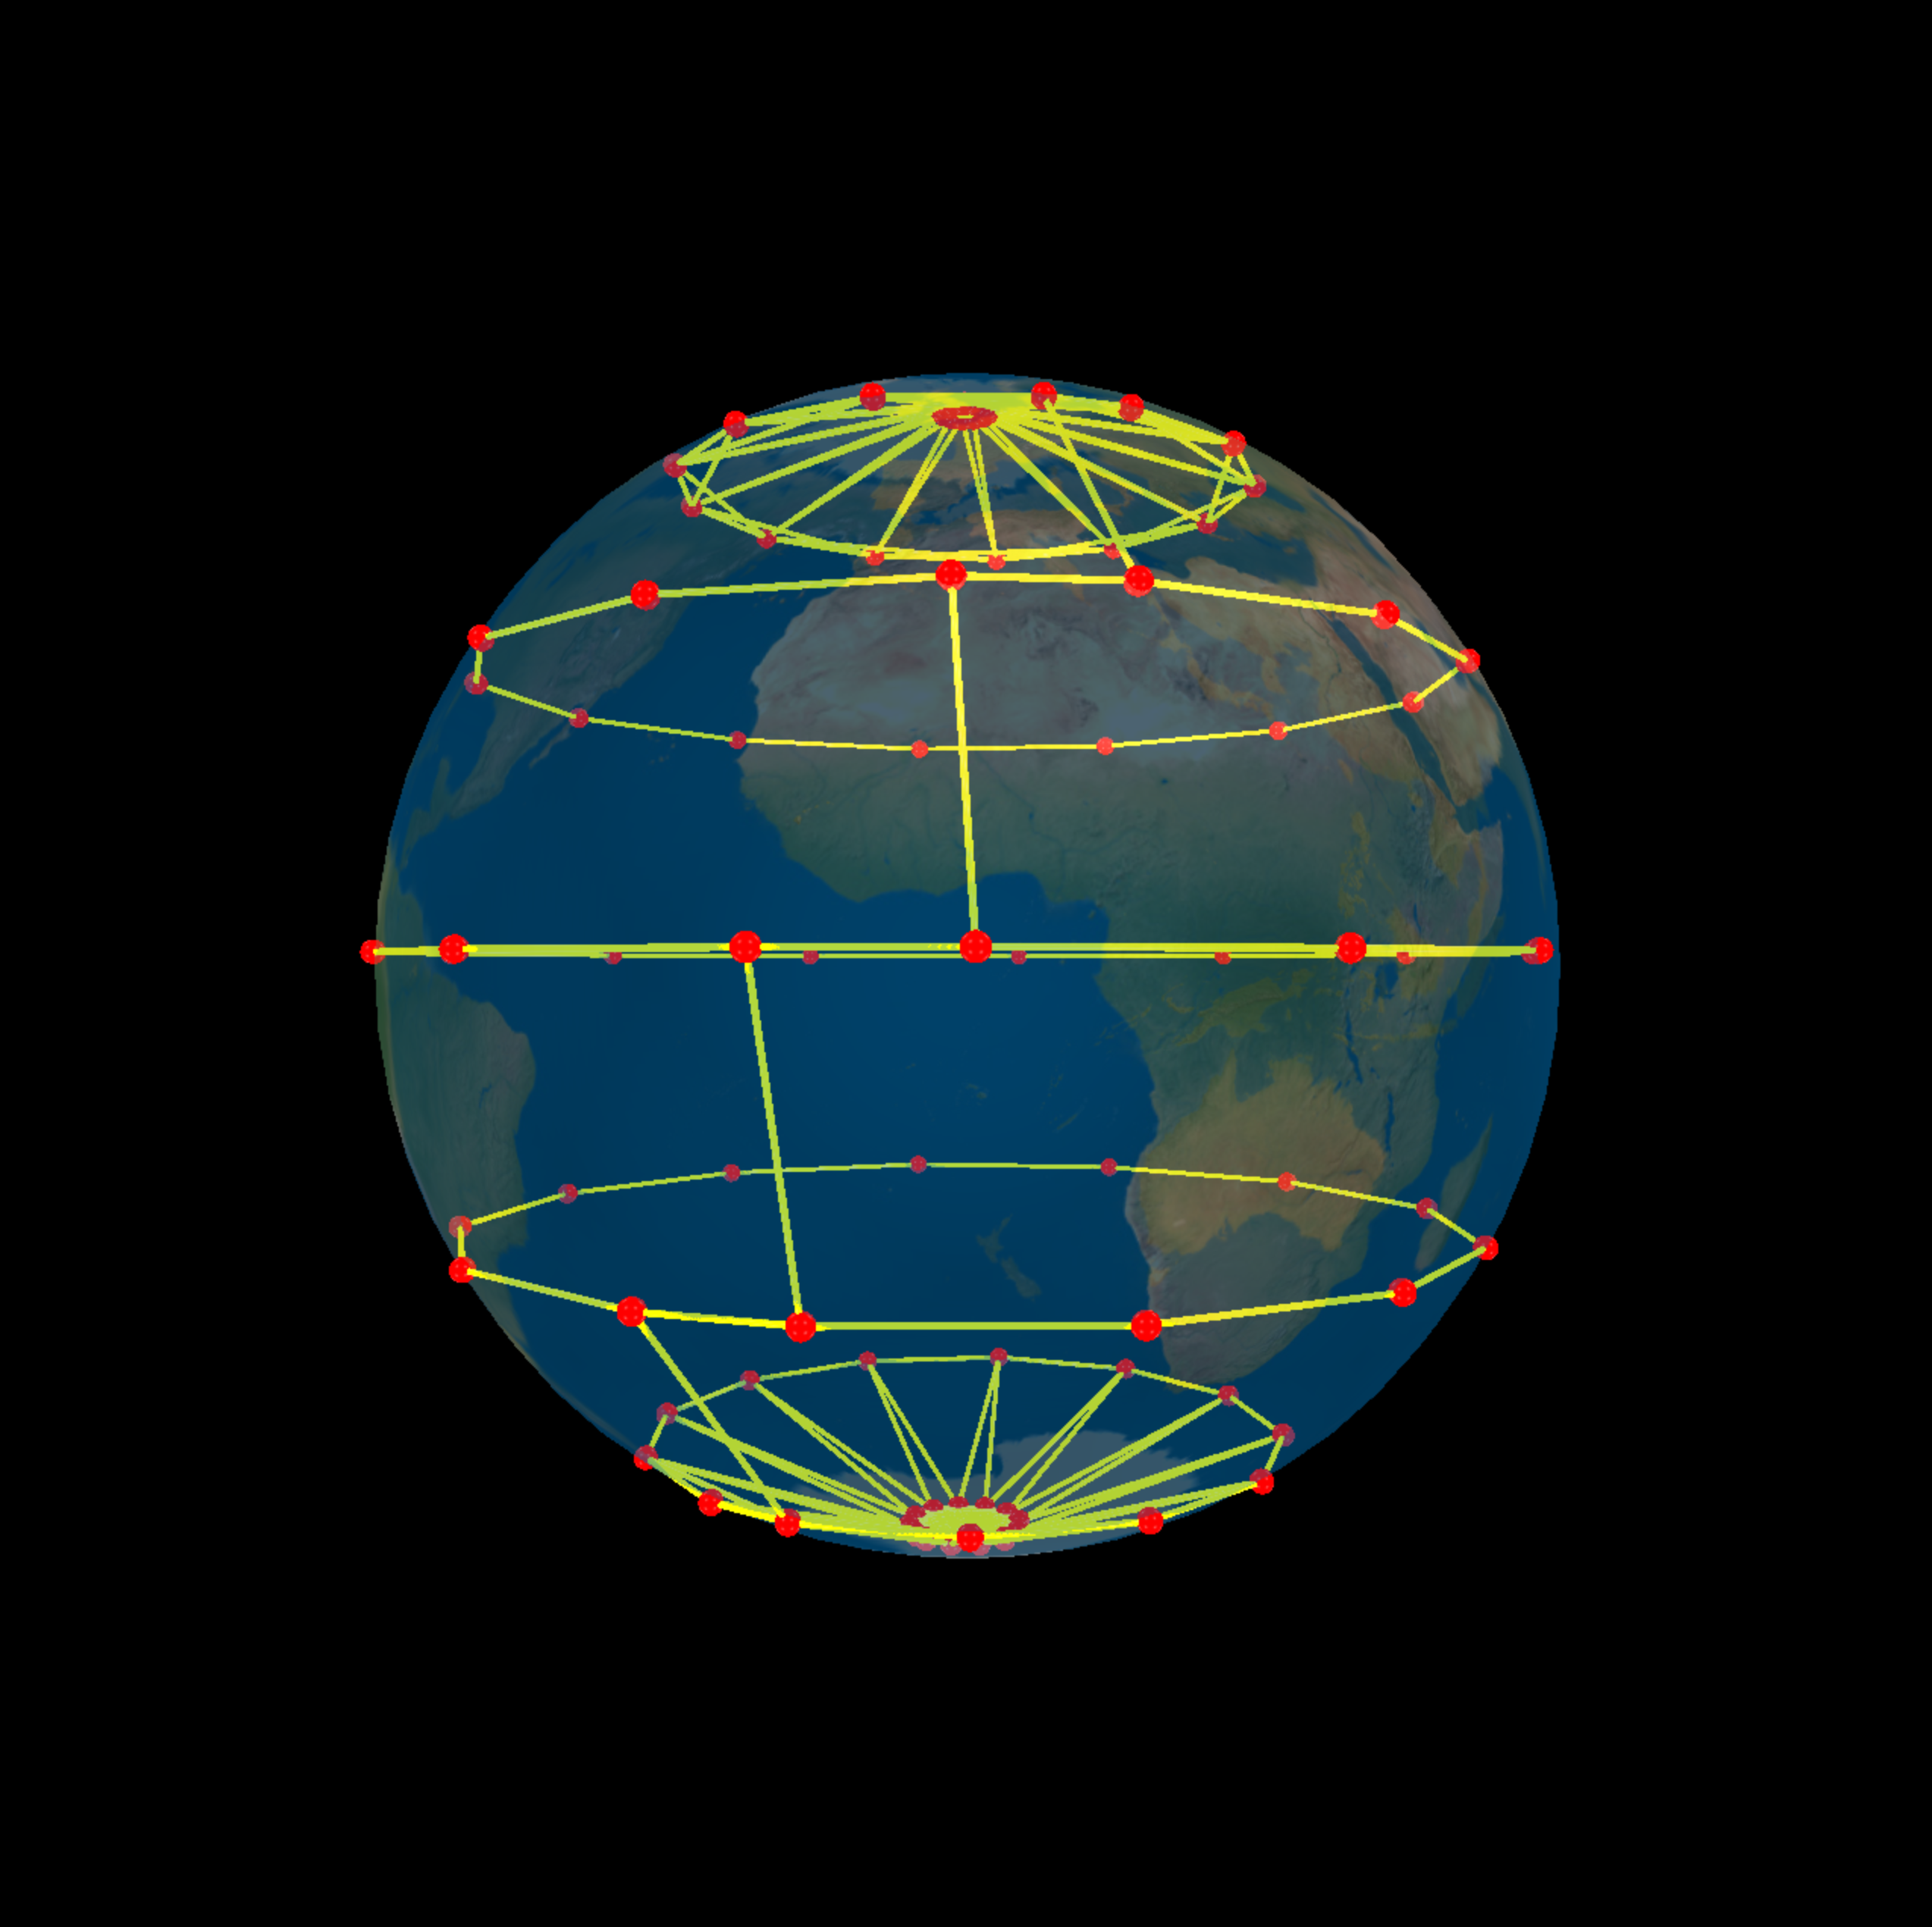
\includegraphics[width=\textwidth]{../images/connections02}
                \caption{sensors02.txt ($r=0.5$)}
            \end{subfigure}
        }
        \caption{Connections between sensors}
\end{figure}

\section{Coverage}
TODO: Cech complex, increasing $r$ until Betti number $b_1$ is 0 (zero cycles/holes). plots (homology, barcode), 3d image

\begin{figure}[H]
        \centering
        \makebox[\linewidth][c]{
        	\centering
            \begin{subfigure}[b]{0.6\textwidth}
                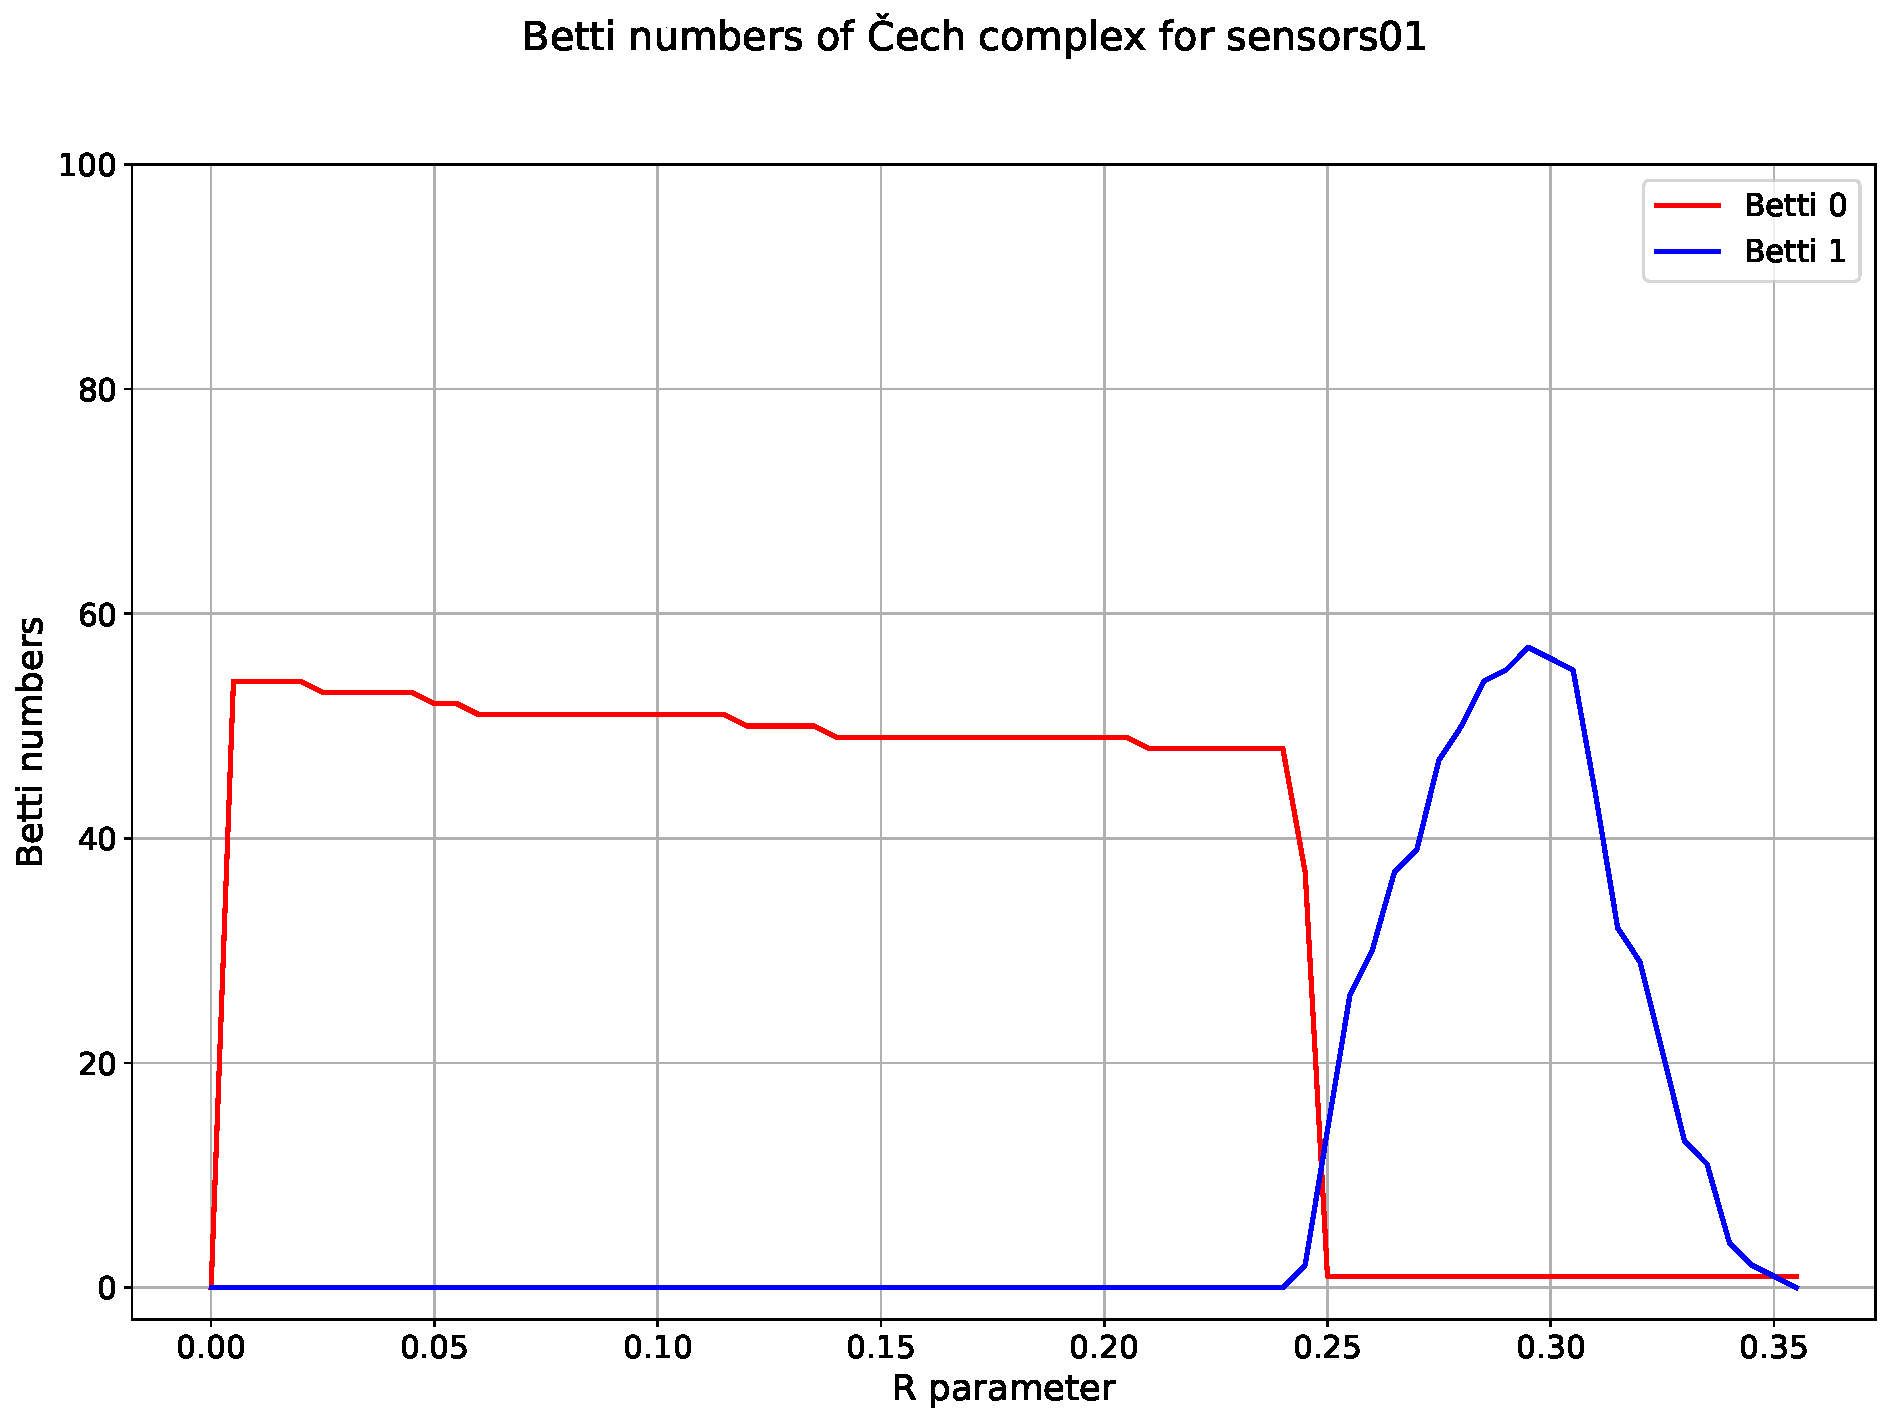
\includegraphics[width=\textwidth]{../images/plot_cech_sensors01}
            \end{subfigure}
            \begin{subfigure}[b]{0.6\textwidth}
                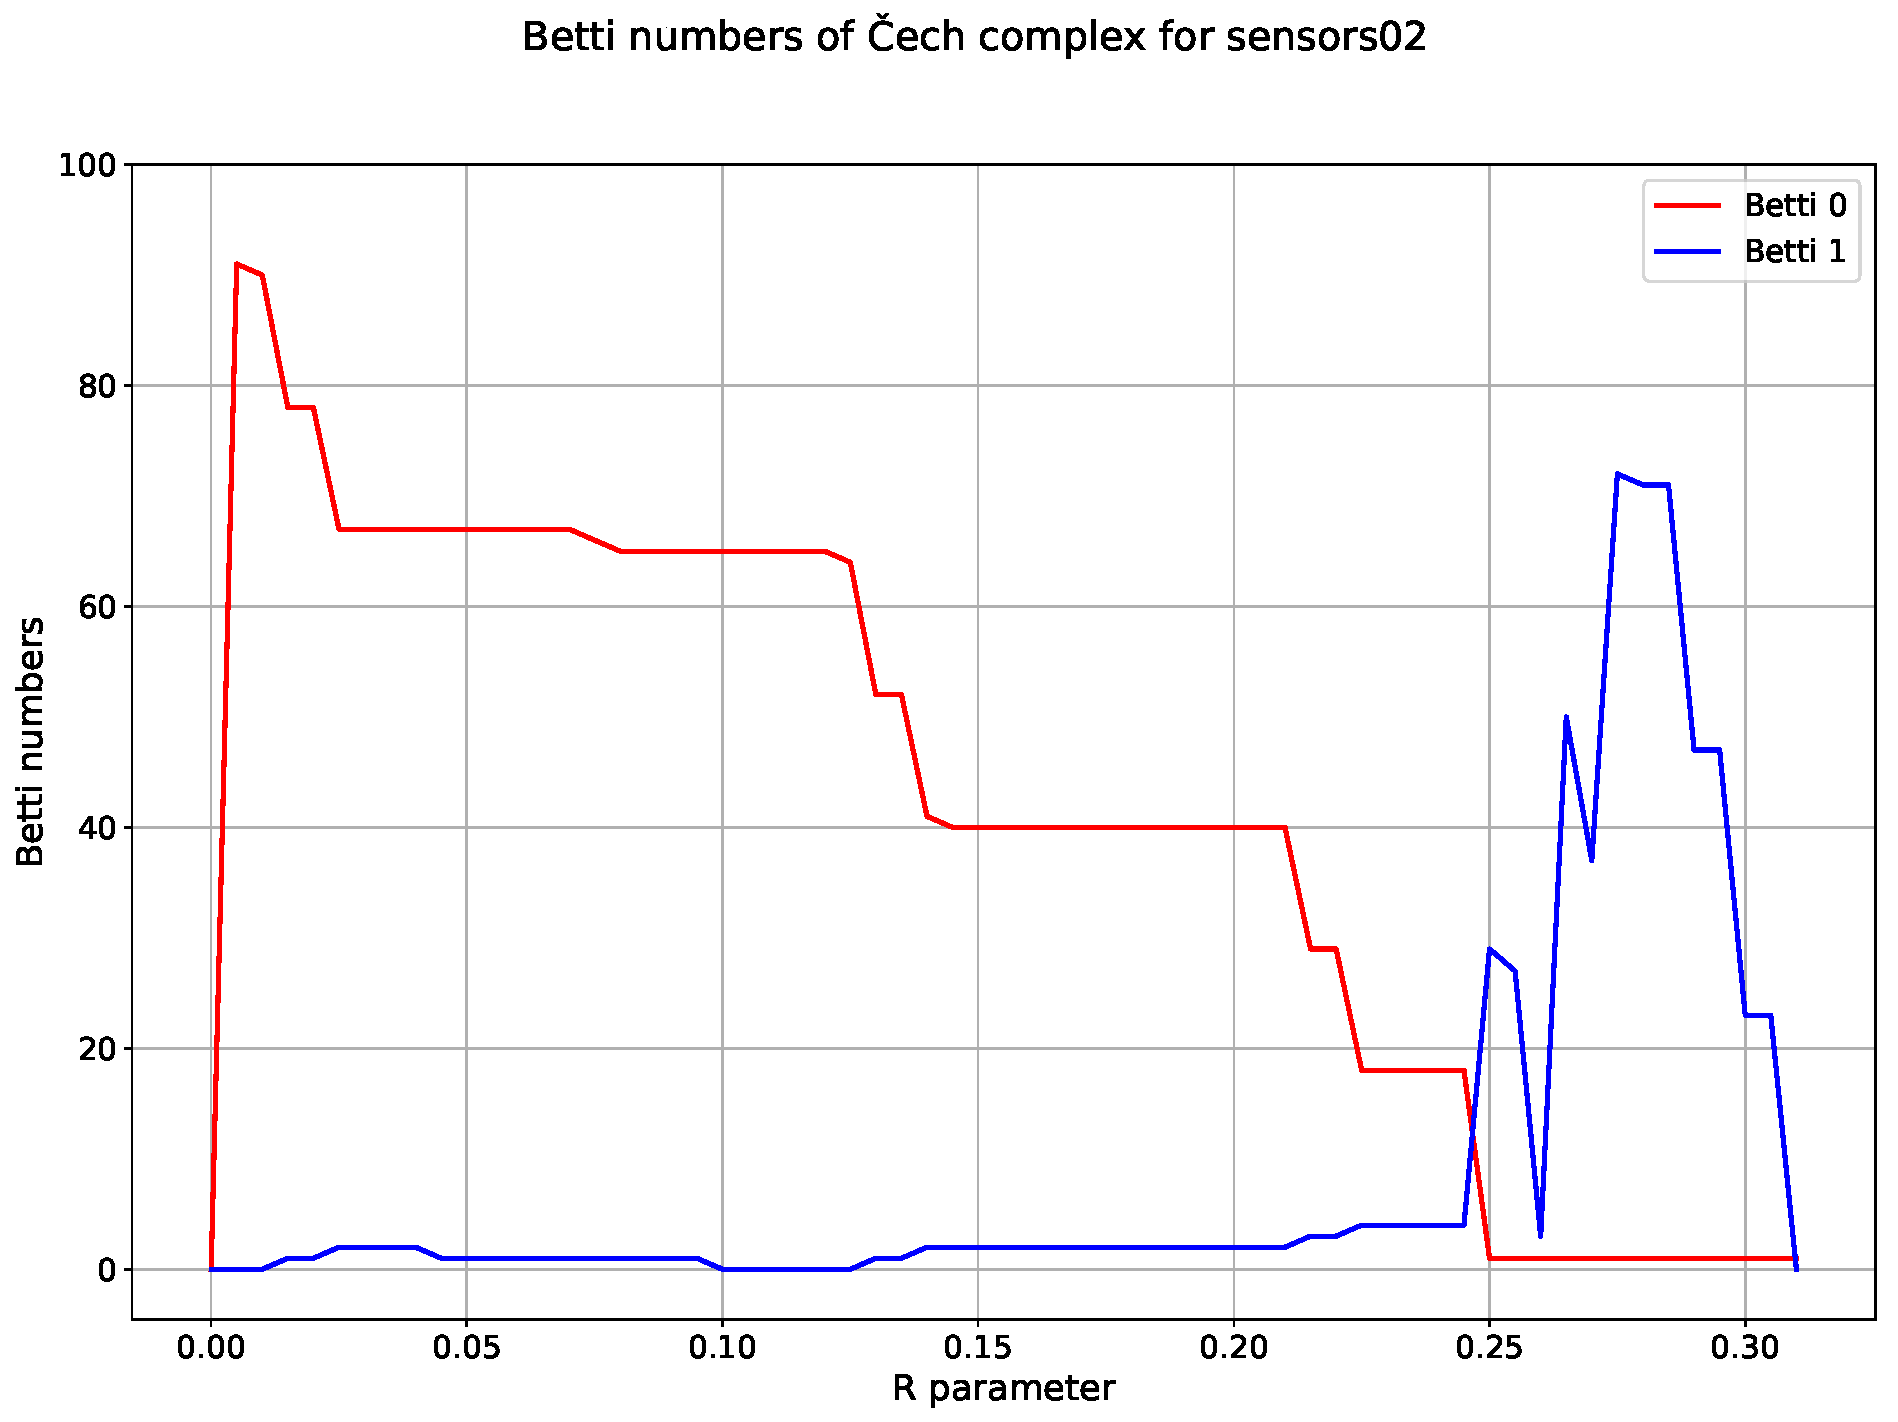
\includegraphics[width=\textwidth]{../images/plot_cech_sensors02}
            \end{subfigure}
        }
        \caption{$b_0$ and $b_1$ as we increase the $R$ parameter}
\end{figure}

\begin{figure}[H]
        \centering
        \makebox[\linewidth][c]{
            \centering
        	\begin{subfigure}[b]{0.6\textwidth}
            	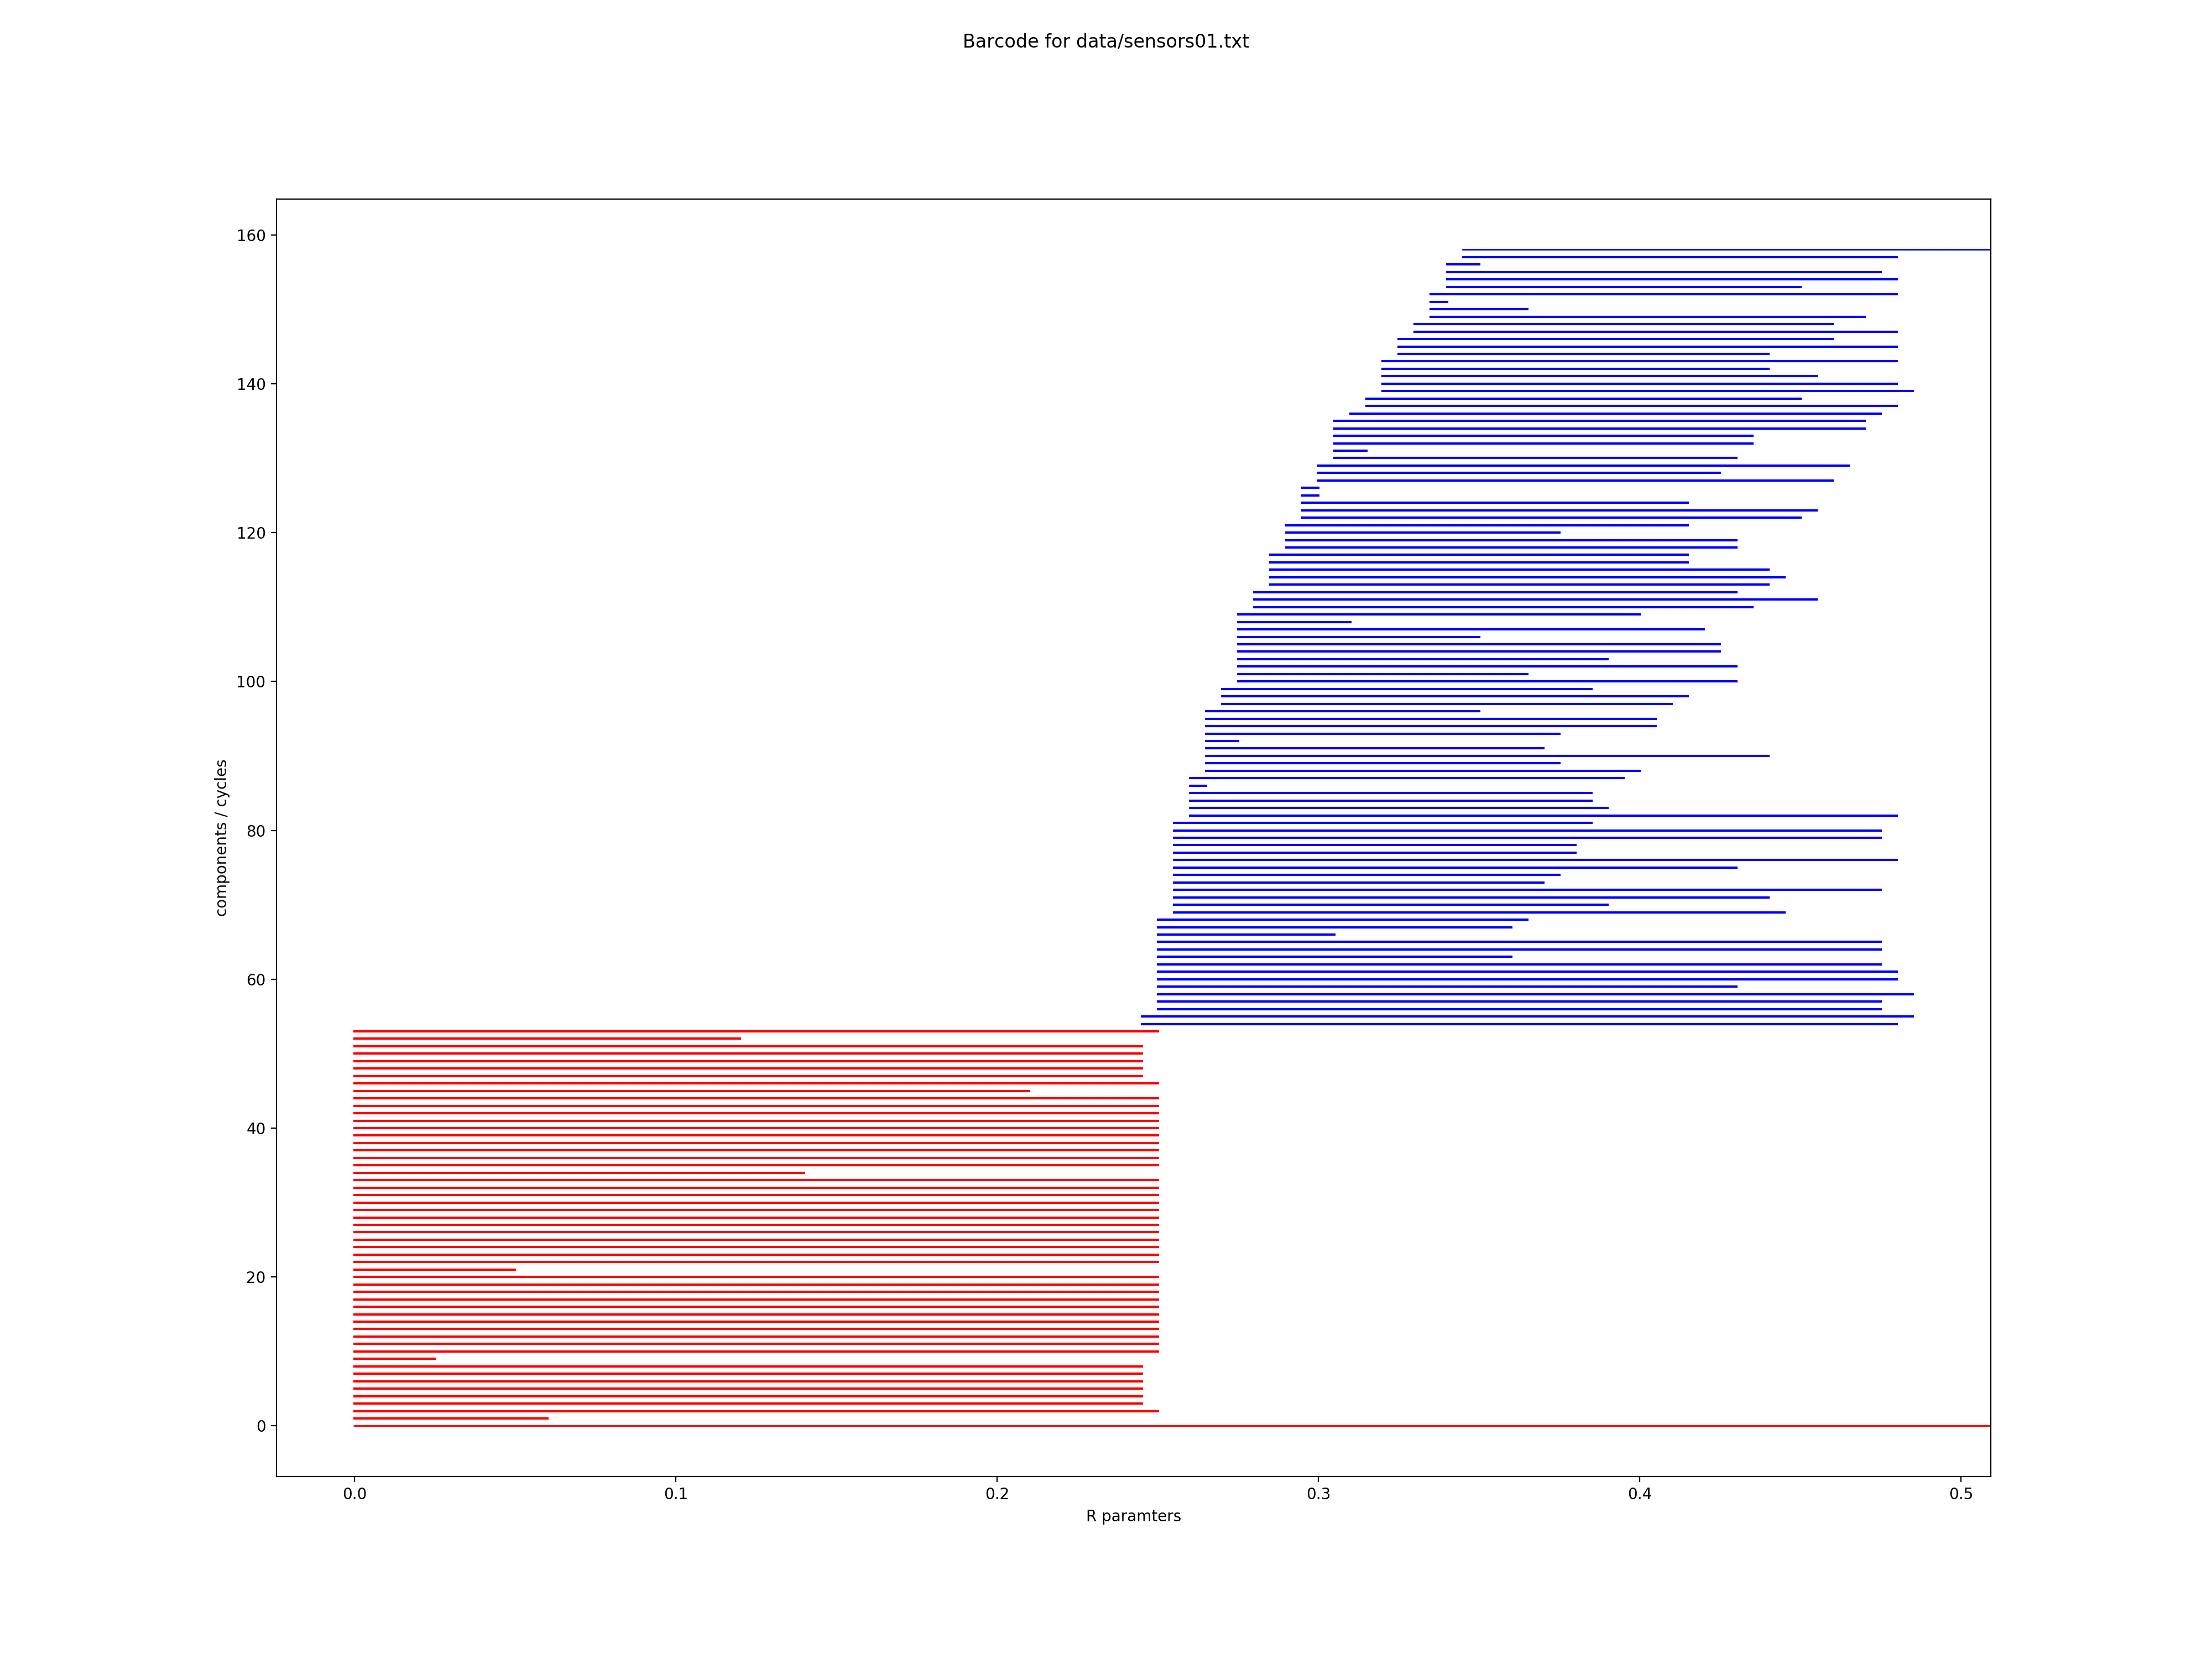
\includegraphics[width=\textwidth]{../images/barcode_cech_sensors01}
        	\end{subfigure}
			\begin{subfigure}[b]{0.6\textwidth}
            	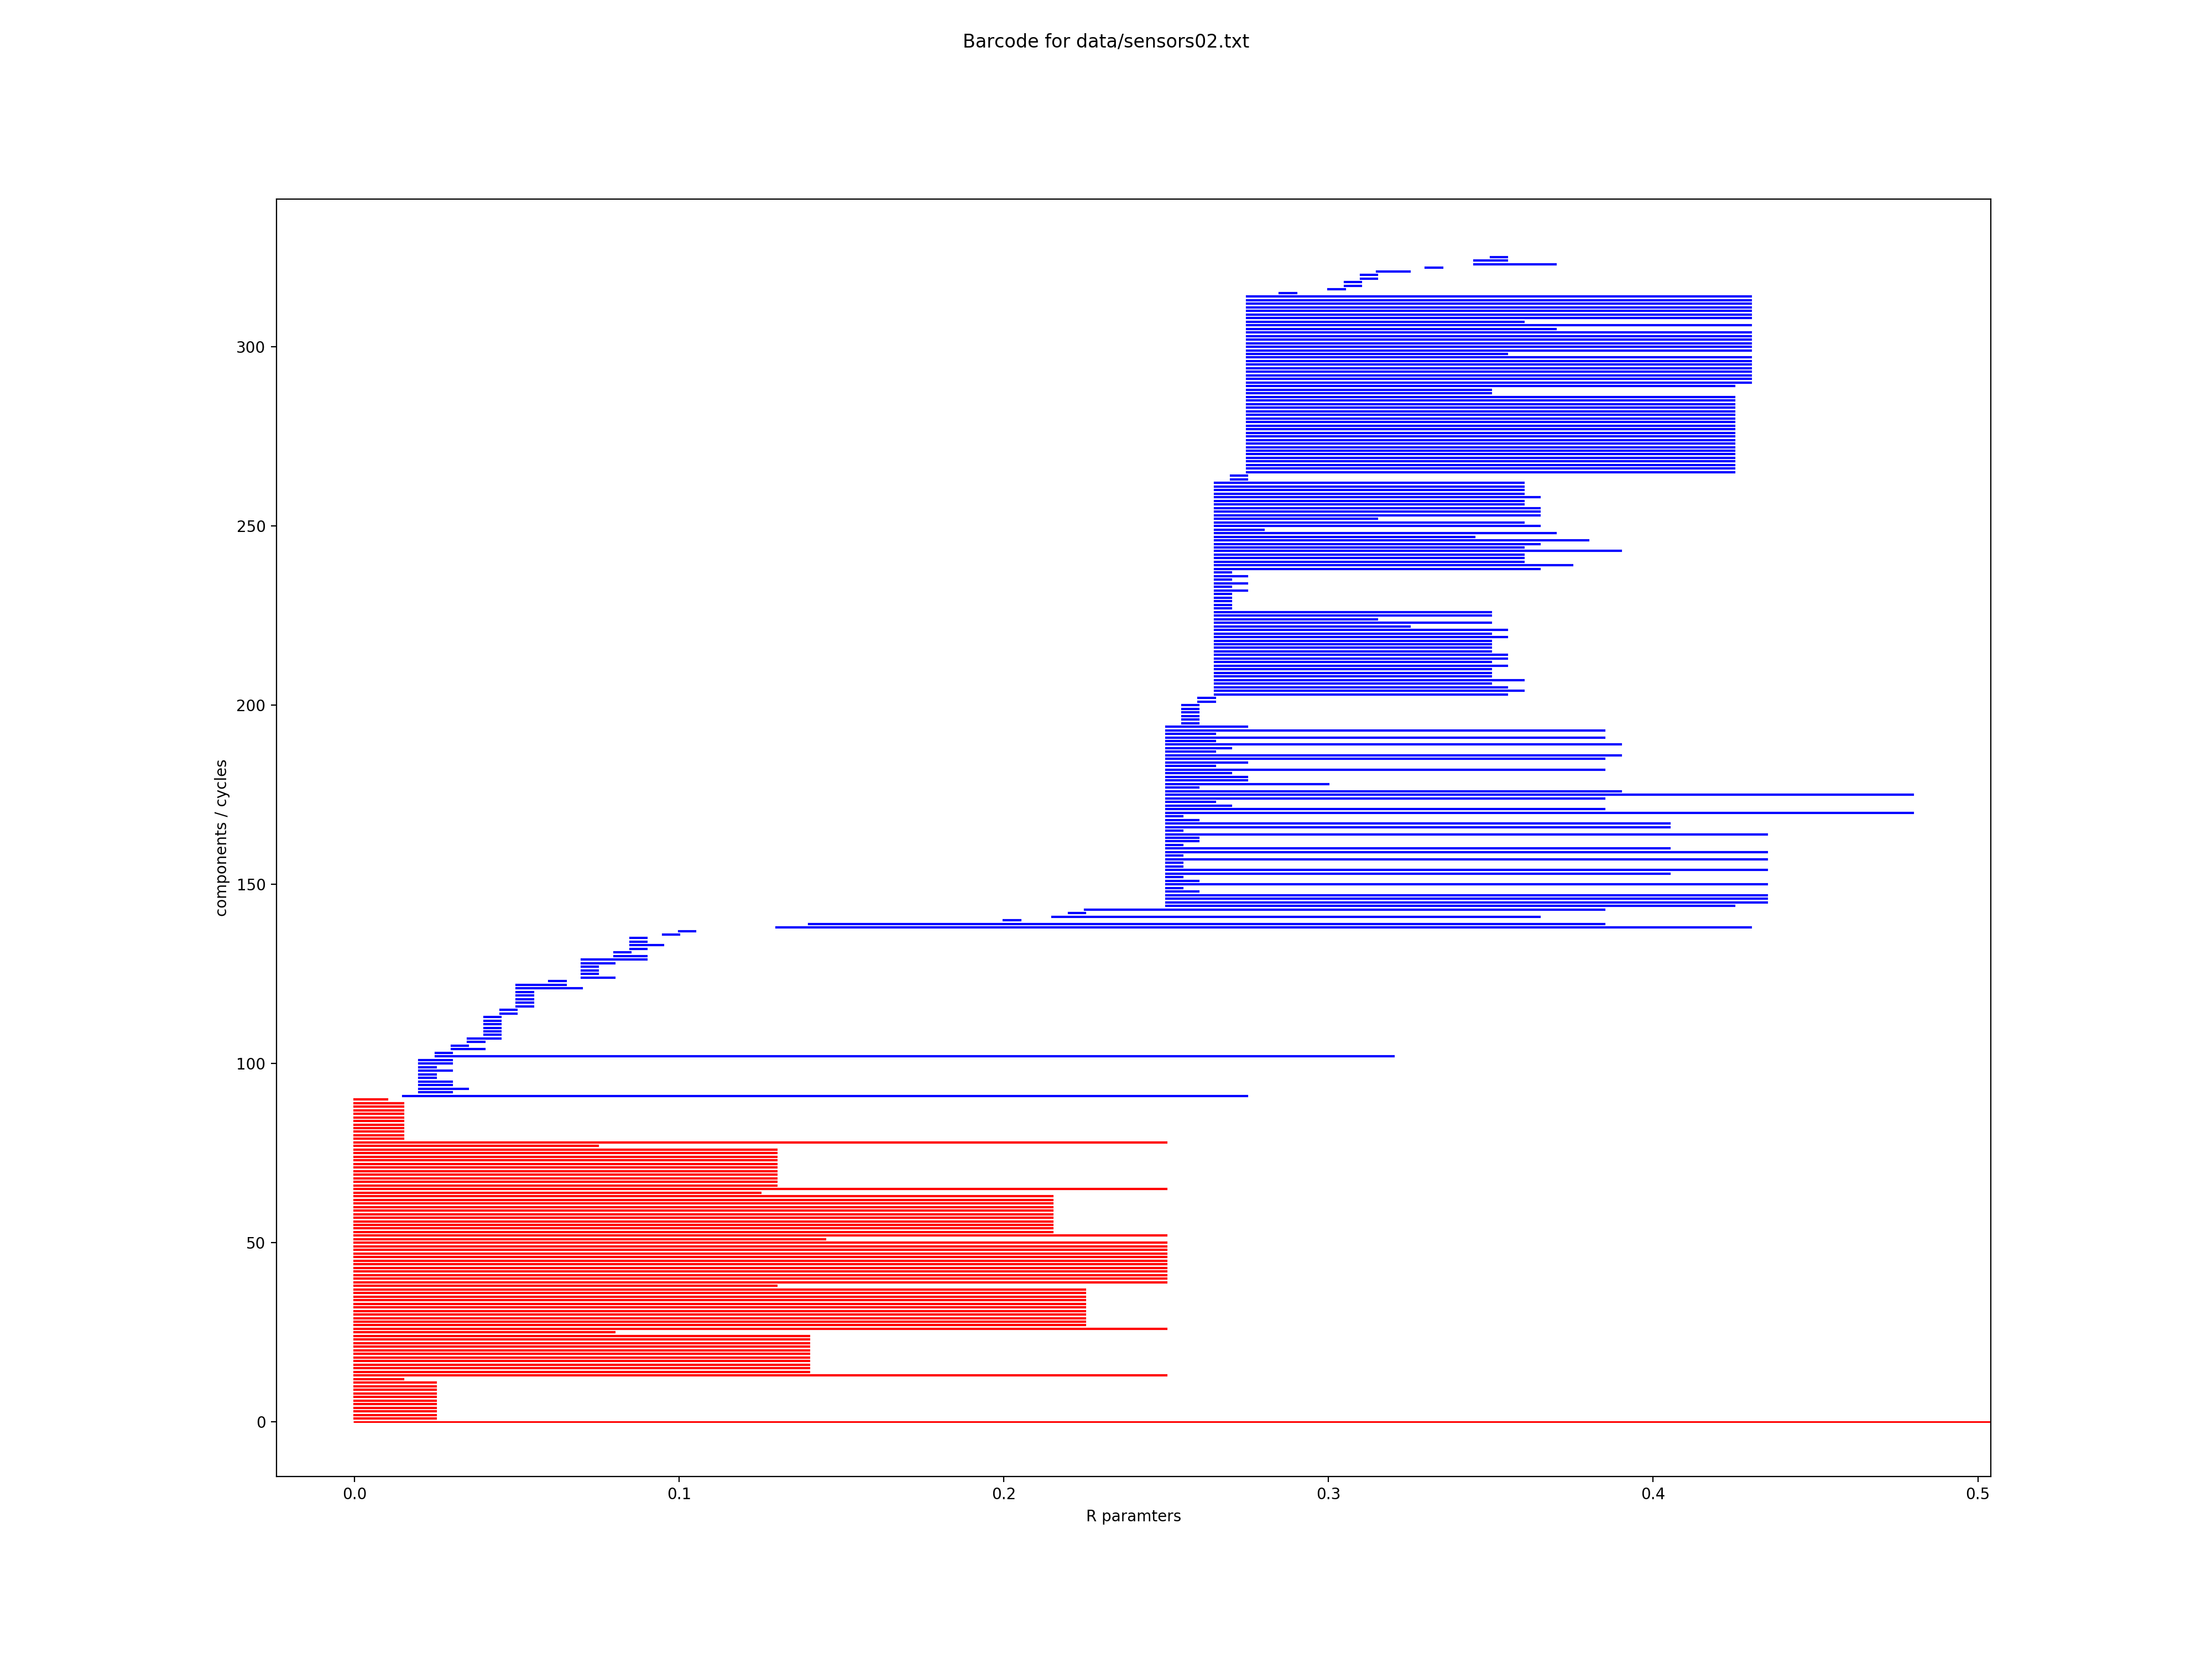
\includegraphics[width=\textwidth]{../images/barcode_cech_sensors02}
        	\end{subfigure}
        }
        \caption{Barcodes for the Čech complex}
\end{figure}

TODO: malo komentarja na graf

\begin{figure}[H]
        \centering
        \makebox[\linewidth][c]{
        	\centering
            \begin{subfigure}[b]{0.55\textwidth}
        	    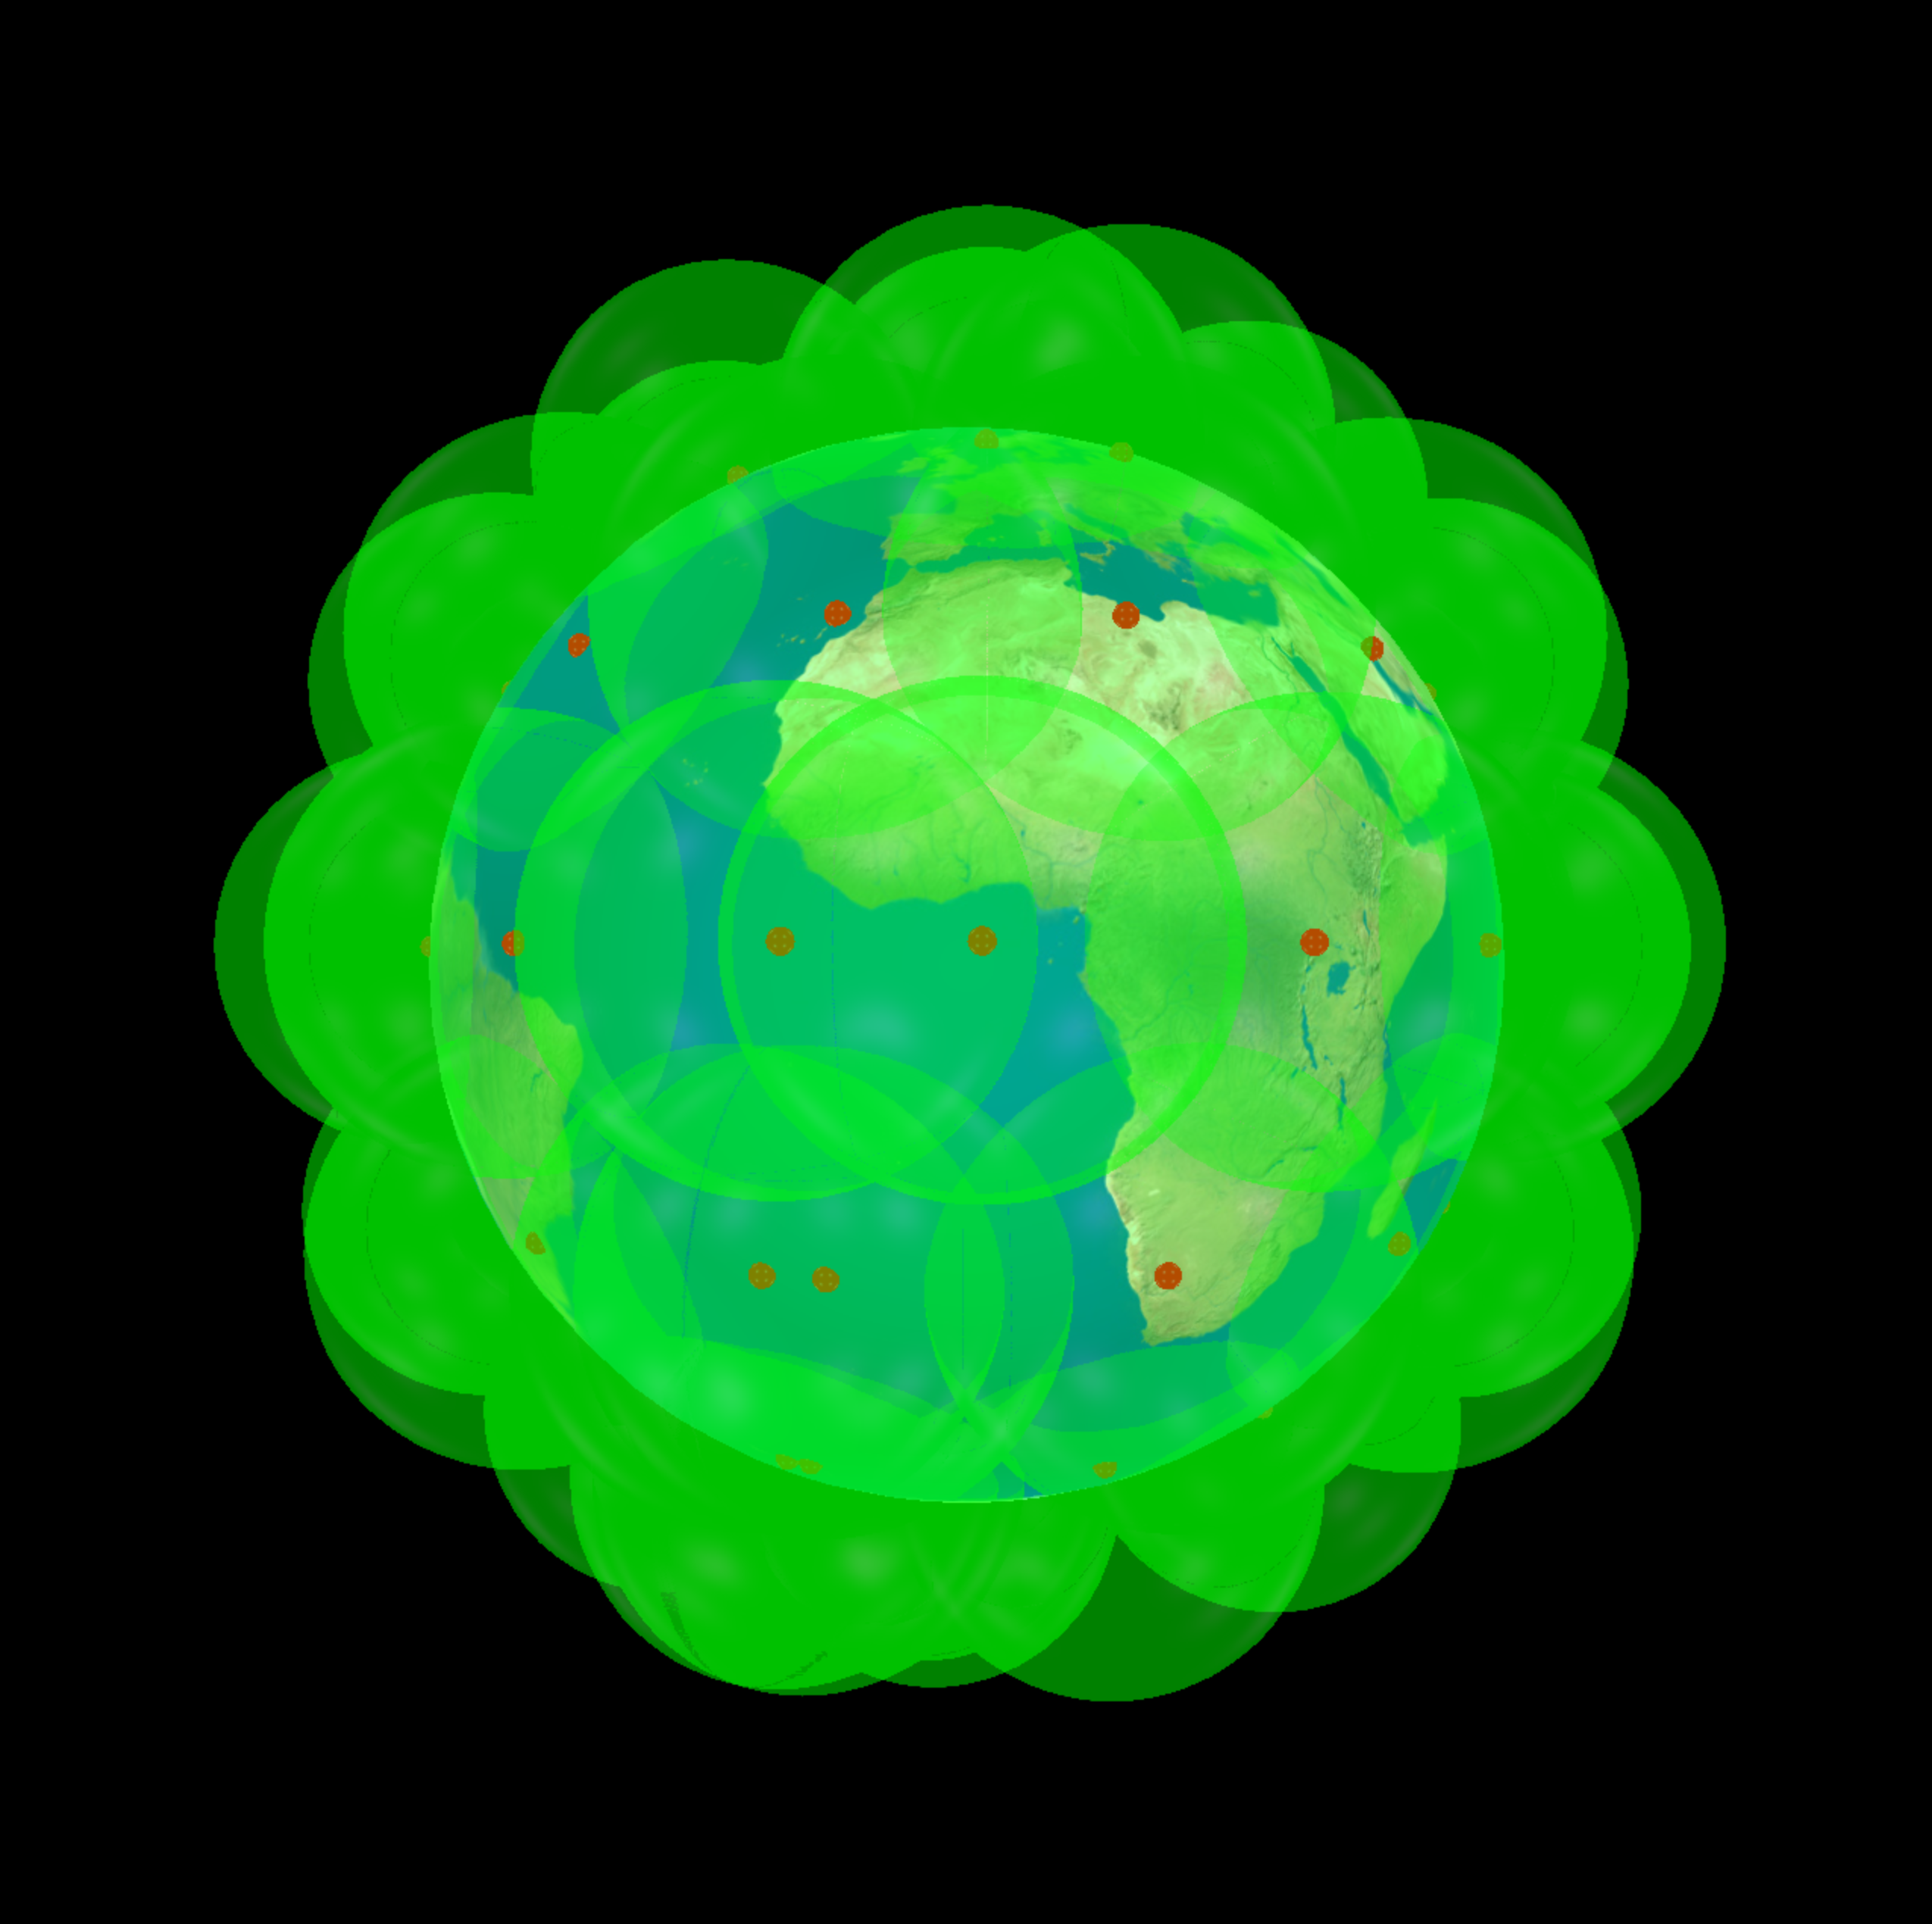
\includegraphics[width=\textwidth]{../images/coverage01}
        	    \caption{sensors01.txt ($R=0.355$)}
        	\end{subfigure}
        	\begin{subfigure}[b]{0.55\textwidth}
      	      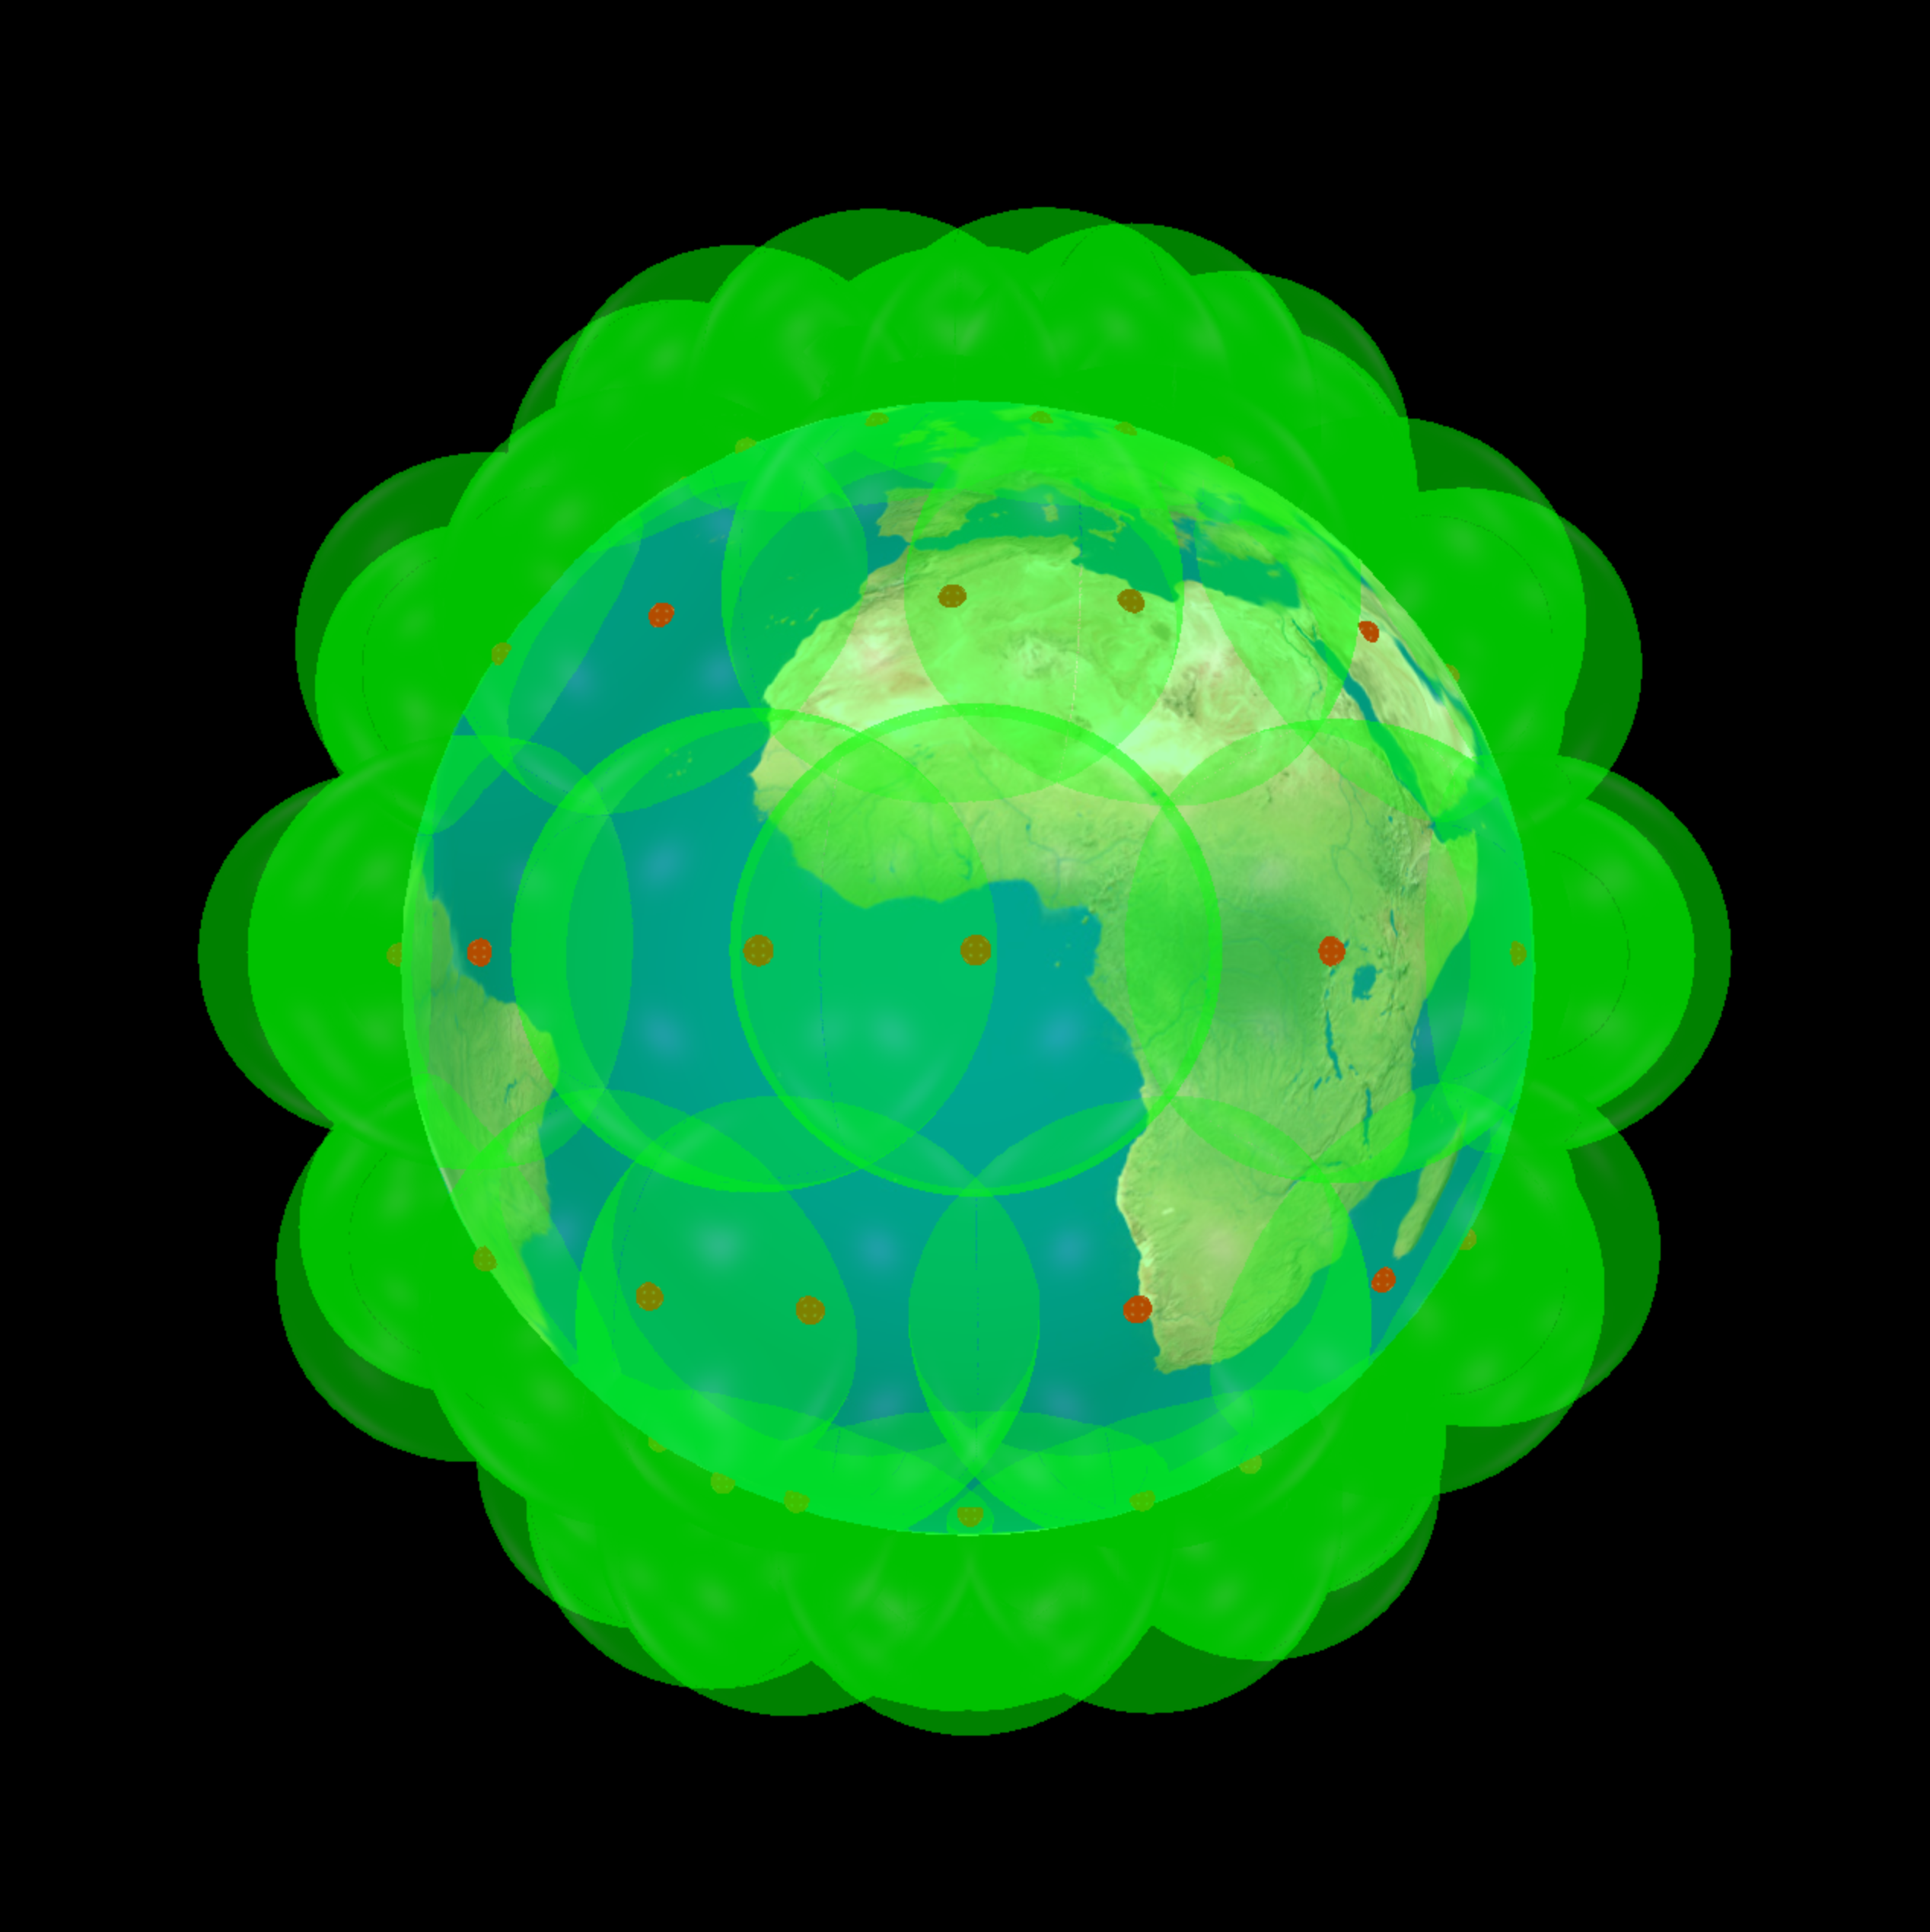
\includegraphics[width=\textwidth]{../images/coverage02}
     	       \caption{sensors02.txt ($R=0.31$)}
     	   \end{subfigure}
	  	}
        \caption{Connections between sensors}
\end{figure}

\section{Data generator}
TODO: data generator

\section{Redundant sensors}
TODO: how we remove the sensors which are not needed

\section{Conclusion}
TODO

\section{References}
Mogoce napiseva samo nestandardne libraryje? dionysus, miniball, vpython Pa link na github

\end{document}
